%!TEX root = kdv.tex
%%%%%%%%%%%%%%%%%%%%%%%
\section{Discretization and numerical results}
%%%%%%%%%%%%%%%%%%%%%%%
\label{secnum}
This section is devoted to the discretization of the optimization problem \eqref{cost} - \eqref{kdvcontrol3}, as well as some insights into the numerical optimization process we use.
\subsection{Discretization of state and adjoint equation}
One difficulty arising when it comes to the discretization of the \KdVB equation is the variety of temporal scales. While the effects of the nonlinearity are only visible after a long time interval, the linear part involves a wide range of scales: the third order derivative represents in particular a high frequency term. In the case of bounded domains numerous schemes are available, be it finite differences \cite{djidjeli1995numerical,zabusky1965interaction}, finite elements \cite{winther1980conservative,arnold1982superconvergent}, finite volumes \cite{dutykh2013finite}, discontinuous Galerkin schemes \cite{Bona1986859,yan2002local}, or polynomial spectral methods \cite{ma2000legendre,ma2001optimal,shen2003new}. One of the most recent and efficient method for the Korteweg-de Vries equation is proposed in \cite{ma2000legendre}. The linear term is treated by a Petrov-Galerkin method (better suited for nonsymmetric problems) on Legendre polynomials, while the nonlinear term is treated pseudospectrally on Chebyschev collocation points. Shortly after, Shen \cite{shen2003new} proposed an improvement of this Petrov-Galerkin method with nearly optimal computational complexity. This will be our method of choice and we recall it here briefly. Since it has never been used on optimal control problem, we also discuss an appropriate discretization of the method regarding the time stepping scheme used.



%Moreover, it is also equivalent to a natural weighted spectral-Galerkin formulation. For those reasons,
%This will be our method of choice and we recall it here briefly. Since it has never been used on optimal control problem, we also discuss an appropriate discretization of the method regarding the time stepping scheme used.

% One of the most recent and efficient discretization method is a pseudospectral Petrov-Galerkin method on Chebyshev collocation points, as introduced in \cite{ma2000legendre}, and improved in \cite{shen2003new}.
%
%  With the aim of tackling an optimal control problem, spectral discretizations present interesting advantages compared to any finite difference or finite element method \cite{boydchebyshev}. First of all they provide very low approximation errors: in some simple cases, these approaches are even exponentially convergent. As a result, the number of grid points required to achieve the desired precision can be very low and the memory needed to store the variables less than for alternative methods. This is a very convenient feature in our perspective, where the optimization part requires the storage of the forward and backward problem in space and time. Finally, there exist nowadays high-performance implementations of the algorithms required to transform bases for most spectral methods. Because of the nonlinearity in the \KdVB equation,
%
%
% TO SUMMARIZE
%
% spectral collocation methods shall be favoured: they indeed allow to represent the variables in terms of their values on a set of points and not only as the coefficients in the spectral expansion. However, for third order equation, the authors show in \cite{merryfield1993properties} that Chebyshev and Legendre collocation methods are unstable. That is why pseudospectral method habe been popular for third order PDEs. Fourier pseudospectral methods have been extensively used \cite{trefethen2000spectral,maday1988error,fornberg1978numerical}. They are in particular very fast when combined with the Fast Fourier Transform to treat the nonlinear term on collocation points. Nevertheless, they are only suited for periodic boundary conditions. Polynomial pseudospectral method on the contrary, which are more adequate for bounded intervals, proved to be stable for the linear third-order differential equation with Chebyshev or Legendre Gauss Lobatto points as collocation points \cite{HuangSloan1992}. They have also demonstrated great performances compared to any other method (see the benchmarking in \cite{skogestad2009boundary}). An interesting hybrid method is proposed in \cite{ma2000legendre}, where the linear term is treated by a Petrov-Galerkin method (better suited for nonsymmetric problems) on Legendre polynomials, while the nonlinear term is treated pseudospectrally using a Chebyshev method. Shortly after, Shen \cite{shen2003new} proposed another dual Petrov-Galerkin method with nearly optimal computational complexity. Moreover, it is also equivalent to a natural weighted spectral-Galerkin formulation. For those reasons, this will be our method of choice and we recall it here briefly. Since it has never been used on optimal control problem, we also discuss an appropriate discretization of the method regarding the time stepping scheme used.

\subsubsection{The dual Petrov-Galerkin method}
The interesting feature of this method lies in the choice of the test and trial functions bases. They are chosen as a compact combination of Legendre polynomials in such a way that the trial functions satisfy the underlying boundary conditions of the equation and the test functions satisfy the dual boundary conditions. Therefore, most matrices involved in the resolution of the problem are sparse or well-conditioned. We present the method for some reference domain $[-1,1]$, but it can be extended to any other domain of type $[a,b]$ by carefully scaling the Legendre polynomials and the integrals. We denote by $P_N$ the space of polynomials of degree $\leq N$ and set
\be
V_N = \left\{y\in P_N : y(1)=y(-1)=\partial_x y(1)=0\right\},
\ee
\be
V_N^{\ast} = \left\{y\in P_N : y(1) = y(-1) = \partial_x y(-1)=0\right\}.
\ee
We consider then the semi-discrete problem: find 
\beal\nonumber 
y_N: \quad &I \rightarrow V_N\\
&t \mapsto y_N(t)
\eeal
\begin{multline}
\left(\partial_t y_N , \varphi_N\right) - \left( y_N, \partial_x \varphi_N \right) + \left(\partial_x y_N, \partial_{xx}\varphi_N \right)  + \\ \gamma \left( \partial_x y_N, \partial_x \varphi_N \right)- \left(\frac{y_N^2}{2}, \partial_x \varphi_N\right)= \langle u, \varphi_N\rangle, \quad \forall v_N \in V_N^{\ast},
\label{petrovgalerkin}
\end{multline}
where $\left( \cdot, \cdot \right)$ denotes the usual $L^2(\Omega)$ spatial inner product and $\langle \cdot, \cdot \rangle$ is the spatial duality pairing between $H^{-1}(\Omega)$ and $H^1_0(\Omega)$, as in the continuous case.
Denoting by $L_k$ the $k$th Legendre polynomial, we can define the basis functions as follows (see Figure~\ref{basisfunctions})
\be
\phi_k(x) = L_k(x) - \frac{2k+3}{2k+5}L_{k+1}(x) - L_{k+2}(x) + \frac{2k+3}{2k+5}L_{k+3}(x),
\ee
\be
\psi_k(x) = L_k(x) + \frac{2k+3}{2k+5}L_{k+1}(x) - L_{k+2}(x) - \frac{2k+3}{2k+5}L_{k+3}(x).
\ee
\begin{figure}[h!]
\begin{center}
\begin{tikzpicture}[scale=0.7]
\begin{axis}[title={\Large First test functions},
	xmin=-50,
        xmax = 50,
        ymin = -1.5,
        ymax = 2,
        xlabel=$x$,
        legend entries={
        $\psi_0$,
	$\psi_1$,
	$\psi_2$,
	$\psi_5$,
	$\psi_{10}$,
    },
    legend pos=outer north east,
    legend cell align=left,]
\pgfplotstableread{testbasis.txt}\mydata;
\addplot [ 
           color=red,thick,
         ]
         table
         [
           x expr=\thisrowno{0}, 
           y expr=\thisrowno{1} 
         ] {\mydata};
 \addplot [ 
           color=blue,thick,
         ]
         table
         [
           x expr=\thisrowno{0}, 
           y expr=\thisrowno{2} 
         ] {\mydata};
\addplot [ 
           color=green,thick,
         ]
         table
         [
           x expr=\thisrowno{0}, 
           y expr=\thisrowno{3} 
         ] {\mydata};
\addplot [ 
           color=orange,thick,
         ]
         table
         [
           x expr=\thisrowno{0}, 
           y expr=\thisrowno{4} 
         ] {\mydata};
\addplot [ 
           color=cyan,thick,
         ]
         table
         [
           x expr=\thisrowno{0}, 
           y expr=\thisrowno{5} 
         ] {\mydata};
\end{axis}
\end{tikzpicture}
\hspace{0.5cm}
\begin{tikzpicture}[scale=0.7]
\begin{axis}[title={\Large First trial functions},
	xmin=-50,
        xmax = 50,
        ymin = -1.5,
        ymax = 2,
        xlabel=$x$,
        legend entries={
        $\phi_0$,
	$\phi_1$,
	$\phi_2$,
	$\phi_5$,
	$\phi_{10}$,},
    legend pos=outer north east,
    legend cell align=left,]
\pgfplotstableread{trialbasis.txt}\mydata;
\addplot [ 
           color=red,thick,
         ]
         table
         [
           x expr=\thisrowno{0}, 
           y expr=\thisrowno{1} 
         ] {\mydata};
 \addplot [ 
           color=blue,thick,
         ]
         table
         [
           x expr=\thisrowno{0}, 
           y expr=\thisrowno{2} 
         ] {\mydata};
\addplot [ 
           color=green,thick,
         ]
         table
         [
           x expr=\thisrowno{0}, 
           y expr=\thisrowno{3} 
         ] {\mydata};
\addplot [ 
           color=orange,thick,
         ]
         table
         [
           x expr=\thisrowno{0}, 
           y expr=\thisrowno{4} 
         ] {\mydata};
\addplot [ 
           color=cyan,thick,
         ]
         table
         [
           x expr=\thisrowno{0}, 
           y expr=\thisrowno{5} 
         ] {\mydata};
\end{axis}
\end{tikzpicture}

  \caption{Basis functions for the Petrov-Galerkin method.}
\label{basisfunctions}
 \end{center}
\end{figure}


Thus for $N \geq 3$,
\beal
&V_N = \span \left\{ \phi_0,\phi_1,...,\phi_{N-3}\right\},\\
&V_N^{\ast} = \span \left\{ \psi_0,\psi_1,...,\psi_{N-3}\right\}.
\eeal
Then, setting
\beal
& y_N = \sum_{k=0}^{N-3}{\tilde y_k(t)\phi_k},\quad \mathbf{y}(t) = \left( \tilde y_0, \tilde y_1, ..., \tilde y_{N-3}\right)^T\\
& \mathbf{u}(t) = \left( \langle u, \psi_0 \rangle, \langle u, \psi_1 \rangle, ..., \langle u, \psi_{N-3} \rangle\right)^T\\
& m_{ij}=(\phi_j, \psi_i),\quad p_{ij}=-(\phi_j^{'}, \psi_i),\quad q_{ij}=(\phi_j^{'}, \psi_i^{'}),\quad s_{ij}=(\phi_j^{'},\psi_i^{''}),
\label{definitionsmatrices}
\eeal
the variational formulation \eqref{petrovgalerkin} yields
\be
M\frac{d\mathbf{y}}{dt} + \left( -P +\gamma Q  + S \right)\mathbf{y} + F(\mathbf{y}) = \mathbf{u},
\ee
where $M$, $P$, $Q$ and $S$ are matrices of size $(N-2)\times(N-2)$ with coefficients $m_{ij}, p_{ij}, q_{ij}$ and $s_{ij}$. $F(\mathbf{y})$ represents the nonlinear term and it is treated as suggested in \cite{shen2003new} i.e. using the pseudospectral approach. It means that the nonlinearity is evaluated in the spatial domain, that we choose to be the Chebyshev-Gauss-Lobatto(CGL) points, and transfered back in the Legendre spectral space. We therefore need to be able to transform back and forth from the spectral space of Legendre coefficients to the values on the CGL points. This can be done using the fast Fourier transform(FFT) and the Chebyshev-Legendre transform. However, for the polynomial degrees we consider here (between 160 and 512), we rather use the direct method that is faster and easier to handle, especially when it will come to finding a discrete adjoint. We build beforehand the matrices  $L_1 =\left(\phi_j(x_i)\right)$ and $L_2 =\left(\psi_j(x_i)\right)$, $i=1..N+1$, $j=1..N-2$, where the points $x_i$ are the CGL points such that $L_1 \mathbf{y} = (y_N(x_1), y_N(x_2), ...y_N(x_{N+1}))^T$ and the same holds with $L_2$ for a variable in the dual space.

% \subsection{Time stepping scheme and adjoint - Crank-Nicolson}
% We have to deal with a problem of high order derivative. Therefore an explicit temporal discretization would lead to excessively small time steps in order to get stability. An implicit method should rather be considered. In \cite{li2000error}, the authors prove convergence of a pseudospectral method with backward Euler scheme for the \KdV equation. However in practice, the first order accuracy in time authorizes only very small time steps. A second order implicit scheme like the Crank-Nicolson scheme should be preferable, though the resolution of the nonlinear system is computationally demanding. This scheme also has the advantage of being a method of choice in optimal control: using the representation of the Crank-Nicolson scheme as a continuous Galerkin method of degree one (continuous trial linear functions and discontinuous piecewise constant test functions) allows us to give directly the concrete form of the adjoint, tangent and additional adjoint equations leading to the exact computation of the discrete gradient and Hessian \cite{meidner2007adaptive}. Note that the use of discrete derivatives is important for the convergence of our optimization algorithm. The scheme for the state is
%
% \bealn
% &M \tilde y_0=M y_0\\
% &M \tilde y_{n+1} + \frac{\Delta t}{2}\left( (S +\gamma Q -P)\tilde y_{n+1} - F(\tilde y_{n+1})\right)  &=  M \tilde y_{n} + \frac{\Delta t}{2}\left( (S +\gamma Q-P)\tilde y_{n} - F(\tilde y_{n})\right)  \\
%  &  &+ \frac{\Delta t}{2}\left( M\tilde q_n + M \tilde q_{n+1}\right), \quad n=0..N.
% \eealn
%
% Then the discrete adjoint scheme in case of distributed control writes
% %\begin{equation}\left\{
% %\begin{split}
% %M^t p_{N+1} + \frac{\Delta t}{2}\left( (S^t +\gamma Q^t- P^t)p_{N+1} - F'(y_{N+1})^t p_{N+1}\right) = -\frac{\Delta t}{2} A(y_{N+1} - y_d)\\
% % M^t p_{n-1} +  \frac{\Delta t}{2}\left( (S^t  +\gamma Q^t- P^t)p_{n-1}  - F'(y_{n-1})^t p_{n-1}\right)  &= M^t p_{n}\\
% %&- \frac{\Delta t}{2}A((y_{n} - y_d)-(y_{n-1} - y_d))+\frac{\Delta t}{2}\left( (S^t +\gamma Q^t- P^t)p_{n} - F'(y_{n-1})^t p_{n}\right) ,\\
% %&n=2..N+1
% %\end{split}
% %\right.
% %\end{equation}
% \bealn
% &M^t p_{N+1} + \frac{\Delta t}{2}\left( (S^t +\gamma Q^t- P^t)p_{N+1} - F^{'}(y_{N+1})^t p_{N+1}\right) = -\frac{\Delta t}{2} A(y_{N+1} - y_d) \\
% &M^t p_{n-1} +  \frac{\Delta t}{2}\left( (S^t  +\gamma Q^t- P^t)p_{n-1}  - F(y_{n-1})^t p_{n-1}\right)  = M^t p_{n} \\
% & \mbox{\hspace{0.15\textwidth}}- \frac{\Delta t}{2}A((y_{n} - y_d)-(y_{n-1} - y_d) + \frac{\Delta t}{2}\left( (S^t +\gamma Q^t- P^t)p_{n} - F^{'}(y_{n-1})^t p_{n}\right) ,\\
% & \mbox{\hspace{0.6\textwidth}}n=2..N+1\\
% &M^t p_{0}  = M^t p_{1} + \frac{\Delta t}{2}\left( (S^t +\gamma Q^t- P^t)p_{1} - F^{'}(y_{0})^t p_{1}\right)-\frac{\Delta t}{2} A(y_{1} - y_d)
% \eealn
% where the matrix $A = \left( \langle \phi_i,\phi_j\rangle\right)$ comes from the discretization of the Lagrangian (in particular the $L^2$ norm in the cost function). We also give the case of the terminal observations problem because we will use it in our numerical examples.
% \bealn
% & M^t p_{N+1} + \frac{\Delta t}{2}\left( (S^t +\gamma Q^t- P^t)p_{N+1} - F^{'}(y_{N+1})^t p_{N+1}\right) = - A(y_{N+1} - y_d)\\
% & M^t p_{n-1} + \frac{\Delta t}{2}\left( (S^t +\gamma Q^t- P^t)p_{n-1} - F^{'}(y_{n-1})^t p_{n-1}\right)  = M^t p_{n} + \\
% & \mbox{\hspace{0.35\textwidth}}\frac{\Delta t}{2}\left( (S^t +\gamma Q^t- P^t)p_{n} - F^{'}(y_{n-1})^t p_{n}\right), \, n=2..N+1\\
% &M^t p_{0}  = M^t p_{1} + \frac{\Delta t}{2}\left( (S^t +\gamma Q^t- P^t)p_{1} - F^{'}(y_{0})^t p_{1}\right)
%  \eealn

\subsubsection{Discretization of the control $u$}

By $\left\{x_i \right\}, i = 1, 2 ..., N$, we denote the grid points of the spatial mesh (i.e. in our case the CGL points). The control is then discretized as follows
\be
u_N(t) = \sum_{j=1}^{N}{u_j(t)\delta_{x_j}}
\ee
where the functions $u_j(t)$ are pointwise evaluations in time of the control at the grid points and $\delta_{x_j}$ are Dirac functionals located at the grid points. Hence, we clearly have $u_N \in \M$ and can easily define any inner product required in the resolution of the state equation
\be
\langle u_N, \psi \rangle = \sum_{j=1}^{N}{u_j(t)\psi(x_j)}.
\ee
%as well as the norm in the objective functional
%\be
%\|{u_N}\|_{\M} = \sum_{j=1}^N{\left( \sum_{i = 1}^{N_T}{\tau_i u_{ji}^2}\right)^{1/2}},
%\ee
%where $N_T$ is the number of time steps and $\tau_i$ is the size of the $i^{th}$ step. We point out that this precise control discretization was also used and analyzed in \cite{pieper2013priori, pieper2014,casas2013parabolic}.

\subsubsection{Time stepping scheme and adjoint - Crank-Nicolson-Leap-Frog}
We have to deal with a problem of high order derivative. Therefore an explicit temporal discretization would lead to excessively small time steps in order to get stability. An implicit method should rather be considered. In \cite{li2000error}, the authors prove convergence of a pseudospectral method with backward Euler scheme for the \KdV equation. However in practice, the first order accuracy in time authorizes only very small time steps. A second order implicit scheme like the Crank-Nicolson scheme should be preferable. This scheme has the advantage of being a method of choice in optimal control: using the representation of the Crank-Nicolson scheme as a continuous Galerkin method of degree one (continuous trial linear functions and discontinuous piecewise constant test functions) allows us to give directly the concrete form of the adjoint, tangent and additional adjoint equations leading to the exact computation of the discrete gradient and Hessian(see, e.g.\cite{meidner2007adaptive}). Note that the use of discrete derivatives is important for the convergence of our optimization algorithm. However, the Crank-Nicolson scheme is computationally demanding. An alternative is then the two-steps Crank-Nicolson Leap Frog method. In this setting, the third derivative is treated implicitely and the nonlinear term is treated explicitely. This method has already been extensively used for the \KdV equation \cite{shen2003new,ma2000legendre,ma2001optimal}, showing for instance extended stability intervals with the Fourier spectral method \cite{chan1985fourier}. However, to the authors' knowledge, this has never been used in the context of an optimal control problem. Commonly, this method is initialized by a semi-implicit step. We suggest also a slight modification of the last step of this two-steps method in order to get a discrete adjoint that is consistent with the continuous adjoint in both the distributed control problem or the terminal observations problem. The time interval is devided into $N_{T}+1$ steps $0 = t_0 < t_1....< t_{N_{T}} = T$. While the first and last one have length $\frac{\Delta t}{2}$, the other steps are of equal length $\Delta t$. We denote hereafter
$\mathbf{y}_n = \mathbf{y}(t_n) = \left( \tilde y_0(t_n), \tilde y_1(t_n), ..., \tilde y_{N-3}(t_n)\right)^T$
and
$\mathbf{u}_n = \mathbf{u}(t_n) = \left( \langle u(t_n), \psi_0 \rangle, \langle u(t_n), \psi_1 \rangle, ..., \langle u(t_n), \psi_{N-3} \rangle\right)^T$, $ n=0 \ldots N_{T}$.
With the help of the matrices defined in \eqref{definitionsmatrices}, the forward scheme is as follows
\bealn
& \frac{1}{2}\left( M+\Delta t S\right) \mathbf{y}_1 = \frac{1}{2}\left( M + \Delta t P + \gamma \Delta t Q \right) \mathbf{y}_0 + \frac{1}{2}\Delta t F(\mathbf{y}_0) + \frac{1}{2}\Delta t \mathbf{u}_0 \\
& \frac{1}{2}\left( M+\Delta t S\right) \mathbf{y}_{n+1} = \frac{1}{2}\left( M - \Delta t S\right) \mathbf{y}_{n-1} +  \Delta t \left( P + \gamma Q\right)\mathbf{y}_n \\
& \mbox{\hspace{0.5\textwidth}}+ \Delta t F(\mathbf{y}_n) + \Delta t \mathbf{u}_n,  \, n=1 \ldots N_{T}-1\\
& M \mathbf{y}_{N_{T}+1} = \frac{1}{2}\left( M \mathbf{y}_{N_{T}} + M \mathbf{y}_{N_{T}-1} \right)+ \frac{1}{2}\Delta t P \mathbf{y}_{N_{T}} + \frac{1}{2}\Delta t F(\mathbf{y}_{N_{T}}) - \frac{1}{2}\Delta t S \mathbf{y}_{N_{T}-1}
\eealn
The first step is semi-implicit. The interior steps are classical CNLF steps. The last step - due to our modification - is not a regular, well-known step, but it is designed in such a way that the discrete adjoint shall be consistent with a CNLF discretization of the continuous adjoint. Notice that as $\Delta t$ vanishes, it becomes just a mean between the two preceding steps.

As for the resolution of the optimization problem, the objective functional writes at the discrete level
\begin{multline}
J_{N,N_{T}}(\mathbf{y}_{0}, \ldots, \mathbf{y}_{N_{T}}, \mathbf{u}_{0}, \ldots, \mathbf{u}_{N_{T}}) = \frac{1}{2}\sum_{i=1}^{N_{T}}{\Delta t \left(\mathbf{y}_{i} - \mathbf{z}_{1,i}\right)^{t}A \left(\mathbf{y}_{i} - \mathbf{z}_{1,i}\right)} + \\ \frac{1}{2}\left(\mathbf{y}_{N_T} - \mathbf{z}_{2}\right)^{t}A \left(\mathbf{y}_{N_T} - \mathbf{z}_{2}\right)
 + \alpha \sum_{j=1}^N{\left( \sum_{i = 1}^{N_T}{\Delta t \mathbf{u}_{ij}^2}\right)^{1/2}}
\label{discrobj}
 \end{multline}

This allows also to define a discrete Lagrangian:
\begin{multline}
\mathcal{L}_{N,N_{T}}(\mathbf{y}_{0}, \ldots, \mathbf{y}_{N_{T}}, \mathbf{u}_{0}, \ldots, \mathbf{u}_{N_{T}},\mathbf{p}_{0}, \ldots, \mathbf{p}_{N_{T}-1}) = J_{N,N_{T}}(\mathbf{y}_{0}, \ldots, \mathbf{y}_{N_{T}}, \mathbf{u}_{0}, \ldots, \mathbf{u}_{N_{T}})  \\
 + \mathbf{p}_0^T\left[ \frac{1}{2}\left( M+\Delta t S\right) \mathbf{y}_1 - \frac{1}{2}\left( M + \Delta t P + \gamma \Delta t Q \right) \mathbf{y}_0 - \frac{1}{2}\Delta t F(\mathbf{y}_0) - \frac{1}{2}\Delta t \mathbf{u}_0 \right]\\
 +\sum_{k=1}^{N_T-2}{\mathbf{p}_k^T\left[
 \frac{1}{2}\left( M+\Delta t S\right) \mathbf{y}_{k+1} - \frac{1}{2}\left( M - \Delta t S\right) \mathbf{y}_{k-1} - \Delta t \left( P + \gamma Q\right)y_k - \Delta t F(y_k) - \Delta t \mathbf{u}_k\right]}\\
 + \mathbf{p}_{N_T-1}^T\left[ M \mathbf{y}_{N_T} - \frac{1}{2}\left( M \mathbf{y}_{N_T-1} + M \mathbf{y}_{N_T-2} \right)- \frac{1}{2}\Delta t P \mathbf{y}_{N_T - 1} - \frac{1}{2}\Delta t F(\mathbf{y}_{N_T-1}) +\frac{1}{2}\Delta t S \mathbf{y}_{N_T-2}\right].
 \label{discrlag}
 \end{multline}

From \eqref{discrlag}, one can classically derive the discrete adjoint, hereafter written in the case of terminal observations, which will be of particular interest in the numerical examples:
 \bealn
 &M^T \mathbf{p}_{N_T-1} = -A(\mathbf{y}_{N_T} - \mathbf{z}_2)\\
 &\frac{1}{2}\left( M^T+\Delta t S^T\right) \mathbf{p}_{N_T-2} = \frac{1}{2}\left( M^T + \Delta t P^T + \gamma \Delta t Q^T \right) \mathbf{p}_{N_T - 1} + \frac{1}{2}\Delta t F^{'}(\mathbf{y}_{N_T - 1})^T \mathbf{p}_{N_T - 1} \\
 &\frac{1}{2}\left( M^T + \Delta t S^T\right)\mathbf{p}_{n-2} = \frac{1}{2}\left( M^T - \Delta t S^T\right)\mathbf{p}_{n} + \Delta t \left( P^T + \gamma Q^T\right)\mathbf{p}_{n-1} + \Delta t F^{'}(\mathbf{y}_{n-1})^T \mathbf{p}_{n-1}, \\
 &\mbox{\hspace{0.7\textwidth}}\quad n=2 \ldots N_T - 1.
 \label{numschemeadj}
\eealn
Classically, it starts with a projection of the tracking term in the state space into the adjoint space. This is followed by a unique semi-implicit step and regular CNLF steps.
% The lagrangian of the problem writes at the continuous level.
% \beal
%   \mathcal{L}(y,q,p) = \frac{1}{2}\norm{y - y_d}_{\lspace}^2 + \alpha \norm{q}_{\M} + <p, By-q>
% \eeal
% Its (almost) discrete counterpart shall be
% \begin{multline}
% L(\bar y, \bar q, \bar p) = \frac{1}{2}(y_{N+1} - y_d)^t A (y_{N+1} - y_d) + \alpha \norm{q}_{\M} \\
% + p_0^t\left[ \frac{1}{2}\left( M+\Delta t S\right) y_1 - \frac{1}{2}\left( M + \Delta t P + \gamma \Delta t Q \right) y_0 - \frac{1}{2}\Delta t F(y_0) - \frac{1}{2}\Delta t M q_0 \right]\\
% +\sum_{k=1}^{N-1}{p_k^t\left[
% \frac{1}{2}\left( M+\Delta t S\right) y_{k+1} - \frac{1}{2}\left( M - \Delta t S\right) y_{k-1} - \Delta t \left( P + \gamma Q\right)y_k - \Delta t F(y_k) - \Delta t M q_k\right]}\\
% +p_N^t\left[ M y_{N+1} - \frac{1}{2}\left( M y_N + M y_{N-1} \right)- \frac{1}{2}\Delta t P y_N - \frac{1}{2}\Delta t F(y_N) +\frac{1}{2}\Delta t S y_{N-1}\right].
% \end{multline}
% Differentiating with respect to $\bar y$ leads
% \begin{multline}
% \delta L(\bar y, \bar q, \bar p)\delta \bar y = \delta y_{N+1}^t A (\delta y_{N+1} - y_d) \\
% + p_0^t\left[ \frac{1}{2}\left( M+\Delta t S\right) \delta y_1 - \frac{1}{2}\left( M + \Delta t P + \gamma \Delta t Q \right) \delta y_0 - \frac{1}{2}\Delta t F'(y_0)\delta y_0\right]\\
% +\sum_{k=1}^{N-1}{p_k^t\left[
% \frac{1}{2}\left( M+\Delta t S\right) \delta y_{k+1} - \frac{1}{2}\left( M - \Delta t S\right) \delta y_{k-1} - \Delta t \left( P + \gamma Q\right)y_k - \Delta t F'(y_k)\delta y_k \right]}\\
% +p_N^t\left[ M \delta y_{N+1} - \frac{1}{2}\left( M \delta y_N + M \delta y_{N-1} \right)- \frac{1}{2}\Delta t P \delta y_N - \frac{1}{2}\Delta t F'(y_N)\delta y_N + \frac{1}{2}\Delta tS\delta y_{N-1}\right]
% \end{multline}
% Symmetry of the scalar product yields, after re-indexing of the terms
% \beal
% \delta L(\bar y, \bar q, \bar p)\delta \bar y &= \delta y_{N+1}^t A (\delta y_{N+1} - y_d) \\
% &+ \left[ \delta y_1^t\frac{1}{2}\left( M+\Delta t S\right)  - \delta y_0^t\frac{1}{2} \left( M + \Delta t P + \gamma \Delta t Q \right) - \delta y_0^t\frac{1}{2}\Delta t F^{'}(y_0)\right]p_0\\
% &+\sum_{k=2}^{N}{\delta y_k^t\left[
% \frac{1}{2}\left( M+\Delta t S\right)^t \right]p_{k-1}}-\sum_{k=0}^{N-2}{\delta y_k^t\left[\frac{1}{2}\left( M+\Delta t S\right)^t \right]p_{k+1}}\\
% &-\sum_{k=1}^{N-1}{\left[ \delta y_k^t \Delta t\left(P^t + \gamma Q^t + F^{'}(y_k)^t\right)\right]p_k}\\
% &+\delta y_{N+1}^t M^t p_N - \delta y_{N-1}^t \frac{1}{2}(M^t - \Delta t S^t)p_N \\
% &-\delta y_{N}^t \left( \frac{1}{2}(M^t + \Delta t P^t + \Delta t F^{'}(y_N)^t) \right)p_N.
% \eeal
% The discrete adjoint scheme is obtained by imposing $\delta L(\bar y, \bar q, \bar p)\delta \bar y = 0$.
 \begin{rmk}
 Without this modification of the last forward step, the discrete adjoint obtained in the case of terminal observation would be
 \bealn
 &\frac{1}{2}(M^T+\Delta t S^T) \mathbf{p}_{N_T-1} = -A(\mathbf{y}_{N_T} - \mathbf{z}_2)\\
 &\frac{1}{2}\left( M^T+\Delta t S^T\right) \mathbf{p}_{N_T-2} =  \left(\Delta t P^T + \gamma \Delta t Q^T \right) \mathbf{p}_{N_T-1} + \Delta t F^{'}(\mathbf{y}_{N_T - 1})^T \mathbf{p}_{N_T - 1} \\
 &\frac{1}{2}\left( M^T + \Delta t S^T\right)\mathbf{p}_{n-2} = \frac{1}{2}\left( M^T - \Delta t S^T\right)p_{n} + \Delta t \left( P^T + \gamma Q^T\right)p_{n-1} \\
 &\mbox{\hspace{0.4\textwidth}}+ \Delta t F^{'}(\mathbf{y}_{n-1})^T p_{n-1}, \quad n=2 \ldots N_T-1.
 \eealn
 The major difference lies in the second step. It does not correspond to a consistent discretization of the continuous adjoint equation: the time derivative is not reconstructed. It results in practice in huge oscillations in time of the adjoint variable.
 \end{rmk}

 \begin{rmk}
  Unlike the other steps, the modification of the last forward step implies the inversion of the matrix $M$, which is typically ill-conditionned. However, this drawback is easily overcome by the use of a regularization term of type $\varepsilon I_d$ with epsilon of order $h^2$, where $h$ is the mean space step.
 \end{rmk}
 
 The advantage of computing the adjoint lies in the following proposition
 \begin{prop}
 Following the definition of the discrete objective functional $J_{N,N_T}$ \eqref{discrobj} and discrete lagrangian $\mathcal{L}_{N,N_T}$ \eqref{discrlag}, the discrete derivative of the reduced tracking cost term is given by $\left(-\mathbf{p}_0,\ldots,-\mathbf{p}_{N_T-1}\right)$, where $\mathbf{p}$ is the discrete adjoint state defined by the numerical scheme \eqref{numschemeadj}.
 \end{prop}
\begin{proof}
 The proof is done by standard differentiation of the discrete Lagrangian.
\end{proof}


\subsection{Numerical treatment of the optimization problem}
\subsubsection{The regularized problem}
Numerically, the optimization problem is solved via a Newton type method. This requires an additional regularization term which we introduce as follows
\beal
\min_{q \in \M} J(y) &= \frac{1}{2}\norm{y - y_d}_{\lspace}^2 + \alpha \norm{u}_{L^1(\Omega,L^2(I))} + \frac{\gamma}{2}\norm{u}_{L^2(\Omega,L^2(I))} \\
& = f(y) + \alpha \norm{u}_{L^1(\Omega,L^2(I))} + \frac{\gamma}{2}\norm{u}_{L^2(\Omega,L^2(I))},
\label{costreg}
\eeal
where $u$ and $y$ are subject to Korteweg-de Vries Burgers equation. This enables us to look for controls in the space $L^2(I\times\Omega)$. Since the embedding $L^1(\Omega,L^2(I))\hookrightarrow \M$ is isometric, then any $y \in L^1(\Omega,L^2(I))$ will satisfy
\be
\psi(u) = \norm{u}_{\M} = \norm{u}_{L^1(I,L^2(\Omega))} = \int_0^L{\norm{u}_{L^2(I)}dx}.
\ee
In \cite{herzog2012directional}, the authors study this problem in the linear case, and prove that this setting promotes a \textit{striped sparsity pattern}. In the nonlinear case, the development is analogous. To obtain the optimality conditions, one introduces the proximal map of the $L^1(\Omega, L^{2}(I))$ norm (see, e.g. \cite{bauschke2011convex}):
\be
Prox_{\gamma\psi}(q)(x) = \frac{1}{\gamma}\left( \gamma - \alpha / \norm{q(x)}_{L^{2}(I)}\right)^{+}q(x) \quad \mbox{ for } q \in L^{2}(\Omega_{c}, L^{2}(I)).
\ee
We can then express the optimality condition for \eqref{costreg} by the pointwise projection formula
\be
\bar u_{\gamma} = -\frac{1}{\gamma}\left( 1 - \alpha/\norm{p_{\gamma}}_{L^{2}(I)}\right)^{+}p_{\gamma}.
\ee
It is then directly possible to solve via a Newton type method the equation
\be
F(u_{\gamma}) = u_{\gamma} + \frac{1}{\gamma}\left( 1 - \alpha/\norm{p_{\gamma}}_{L^{2}(I)}\right)^{+}p_{\gamma} = 0.
\label{optcondition}
\ee
Following \cite{pieperthesis}, one can also reformulate this optimality condition thanks to the "normal map", due to Robinson:
\be
G(q_{\gamma}) = \gamma q_{\gamma} + \nabla f (P_{\gamma}(q_{\gamma})) = 0,
\label{normalmap}
\ee
for an auxiliary variable $q_{\gamma}$ such that $u_{\gamma} = P_{\gamma}(q_{\gamma})$. One easily prove in that case that $q_{\gamma} = -\frac{1}{\gamma} p_{\gamma}$ and equivalence between \eqref{optcondition} and \eqref{normalmap}.

% and we can adapt it to state the following theorem
% \begin{thm}
%  Let $\gamma > 0$. Problem \eqref{costreg} possesses a unique optimal solution  $q_{\gamma} \in L^2(I\times\Omega)$ with corresponding state $y_{\gamma} = S(y_0,q_{\gamma})$ and adjoint state $p_{\gamma} = S'^{\ast}(y_{\epsilon} - y_d)$. The first order optimality condition is the subgradient condition
%  \be
%  -<q - q_{\gamma}, \frac{1}{\gamma}q_{\gamma} + p_{\gamma}> +\alpha \norm{q_{\gamma}}_{L^1(I,L^2(\Omega))} \leq \alpha \norm{q}_{L^1(I,L^2(\Omega))}
%  \ee
%  for all $q \in L^1(I,L^2(\Omega))$. This is summed up in the formula
%  \be
%  u_{\gamma}(t,x) = \gamma\max\left(0,1-\frac{\alpha}{\norm{p_{\gamma}}_{L^2(I)}}\right)p_{\gamma}(t,x)
%  \ee
%  for almost all $(t,x)\in I\times\Omega$.
% \end{thm}
% The idea is then to solve with a semismooth Newton method \cite{ulbrich2002semismooth} the equation
% \be
% F(q_{\gamma}) = q_{\gamma} - \gamma\max\left(0,1-\frac{\alpha}{\norm{p_{\gamma}}_{L^2(I)}}\right)p_{\gamma}(t,x)
% \ee
% In comparison to what is done in \cite{herzog2012directional}, the nonlinearity in our problem requires that we additionally compute the tangent and the second adjoint operators to get the gradient of $F$. Besides, in \cite{pieper2014}, the authors quickly prove that we obtain the original problem in the limiting case for great $\gamma$.
\begin{rmk}
 To solve problem \eqref{normalmap}, we apply a Newton-type method, and since the proximal operator is not differentiable, we use the concept of semismoothness to derive a general derivative for $G$ \cite{ulbrich2002semismooth}. An iterative method (conjugate gradient) is used to solve the Newton system. A globalization strategy is added inspired by the algorithm of truncated conjugate gradient algorithm for trust region problems by Steihaug \cite{pieperthesis,steihaug1983}.
\end{rmk}


\subsubsection{Discretization of the control and mass lumping}
In the unregularized problem, the controls are discretized as nodal Dirac measures. In the regularized case, this is not possible anymore as we need a discretization that is compatible with $L^2(\Omega_c \times I)$ functions. However for this regularized case, one need to find a discretization that should lead to an equivalent problem to \eqref{cost} in the limiting case $\gamma \to 0$ (i.e. to obtain a Dirac measure like discretization). We suggest to follow the strategy in \cite{pieper2014}. The control is discretized in space with piecewise linear, continuous finite elements on a grid whose nodes are the Chebyschev-Gauss-Lobatto points previsously mentionned.

% The finite element space associated with this grid is
% \be
% V_h = \left\{ u_h \in \mathcal{C}_0 (\Omega) \,|\, u_{h|K} \in \mathcal{P}_1(K) \mbox{ for all } K \in \mathcal{T}_h \mbox{ and } u_{h|\partial \Omega} = 0 \right\}.
% \ee
% The discretization parameter h denotes the maximum length of the intervals defined by the CGL points. For the time discretization, we define for any Banach space $V$ the semi-discrete space
% \be
% X_\tau^0 (I,V) = \left\{ v_{\tau} \in L^2(I,V) \, | \, v_{\tau|I_m} \in P_0(I_m,V), m=1..N_T\right\},
% \ee
% where $I_m = (t_{m-1}, t_m]$ and $0 = t_0 < t_1....< t_m = T$. The time steps are denoted $\tau_m = t_m - t_{m-1}$ and by $\tau$ we designate the maximum of them. The full discrete space for the control is then $X_{\tau}^0(I,V_h)$.

Moreover, the various norms involved in the optimization problem shall be computed via mass lumping, i.e, the trapezoidal rule is used for the evaluation of the contributions for each cell. Therefore, for $u_h = \chi_{\Omega_c}\sum_{j=1}^{N_T}{\chi_{I_j}\sum_n{\mathbf{u}_{jn} e_n}}$, it holds
\beal
&\norm{u_h}_{L^1(\Omega_c, L^2(I))} = \sum_{n=1}^N{d_n\left(\sum_{j=1}^{N_T}{\Delta t u_{nj}^2}\right)^{1/2}}, \quad \norm{u_h}_{L^2(\Omega_c, L^2(I))}^2 = \sum_{n=1}^N{d_n\left(\sum_{j=1}^{N_T}{\Delta t u_{nj}^2}\right)},\\
&\langle \chi_{\Omega_c} u_h,\varphi_h \rangle = \sum_{n=1}^N{d_n \sum_{j=1}^{N_T} \Delta t u_{jn}\varphi_{jn}}
\eeal
for all $\varphi_h = \chi_{\Omega_c}\sum_{j=1}^{N_T}{\chi_{I_j}\sum_n{\varphi_{jn} e_n}}$


\subsection{Numerical examples}
The numerical examples illustrate the problem of wave generation. We want to investigate the optimal position and shape of a wavemaker. A similar study has been carried out in a slighty different framework in \cite{nersisyan2014generation}, where one possible applications was to
the design artificial surfing facilities. For that purpose, we use a more physical version of the forced Korteweg-de Vries equation, as the one derived in \cite{milewski2004forced}
\be
\partial_t y + f \partial_x y - \frac{1}{6}\partial_{xxx} y - \frac{3}{2}y \partial_x y = u
\label{PhysicalKDV}
\ee
where the parameter $f$ is proportional to $F-1$ ($F$ is the Froude number). Its value determines if a flow is subcritical ($f\leq 0$) or supercritical ($f> 0 $). The forcing $u$ can be interpreted as the derivative of the bottom topography.


\paragraph{\underline{Inverse problem}.}
In the first example, an inverse problem, we want to find what bottom topography created the waves we observe at a final time T. We generate beforehand a wave on the time period $[0,T]$ with the following source term in a subcritical configuration ($f = -0.5$)

\begin{numcases}
{u(t,x) = }
 \nonumber 10\delta_{\{x = 1.5\}}, \mbox{ when } 0 < t\leq 2.5 \\
 0, \mbox{ when } 2.5 \leq t\leq 5
 \label{forcingq}
\end{numcases}
The spacetime grid is parametrized with $T = 5$, $N = 256$ and $\Delta t = 0.01$ and the result is shown on Fig~\ref{waveobservation}. One can see a series of downstream waves - note that the flow enters the domain from the right - generated by the bottom topography induced by $u$ (recall that $u$ is proportional to the derivative of the topography), while a solitary wave is going upstream, at constant speed and constant height, which is typical for the Korteweg-de Vries equation.. Afterwards, a white Gaussian noise is added to the $y$-profile at final time $T$ such that the magnitude of the noise is in average 5 percent of the magnitude of the original signal.

\begin{figure}[!h]
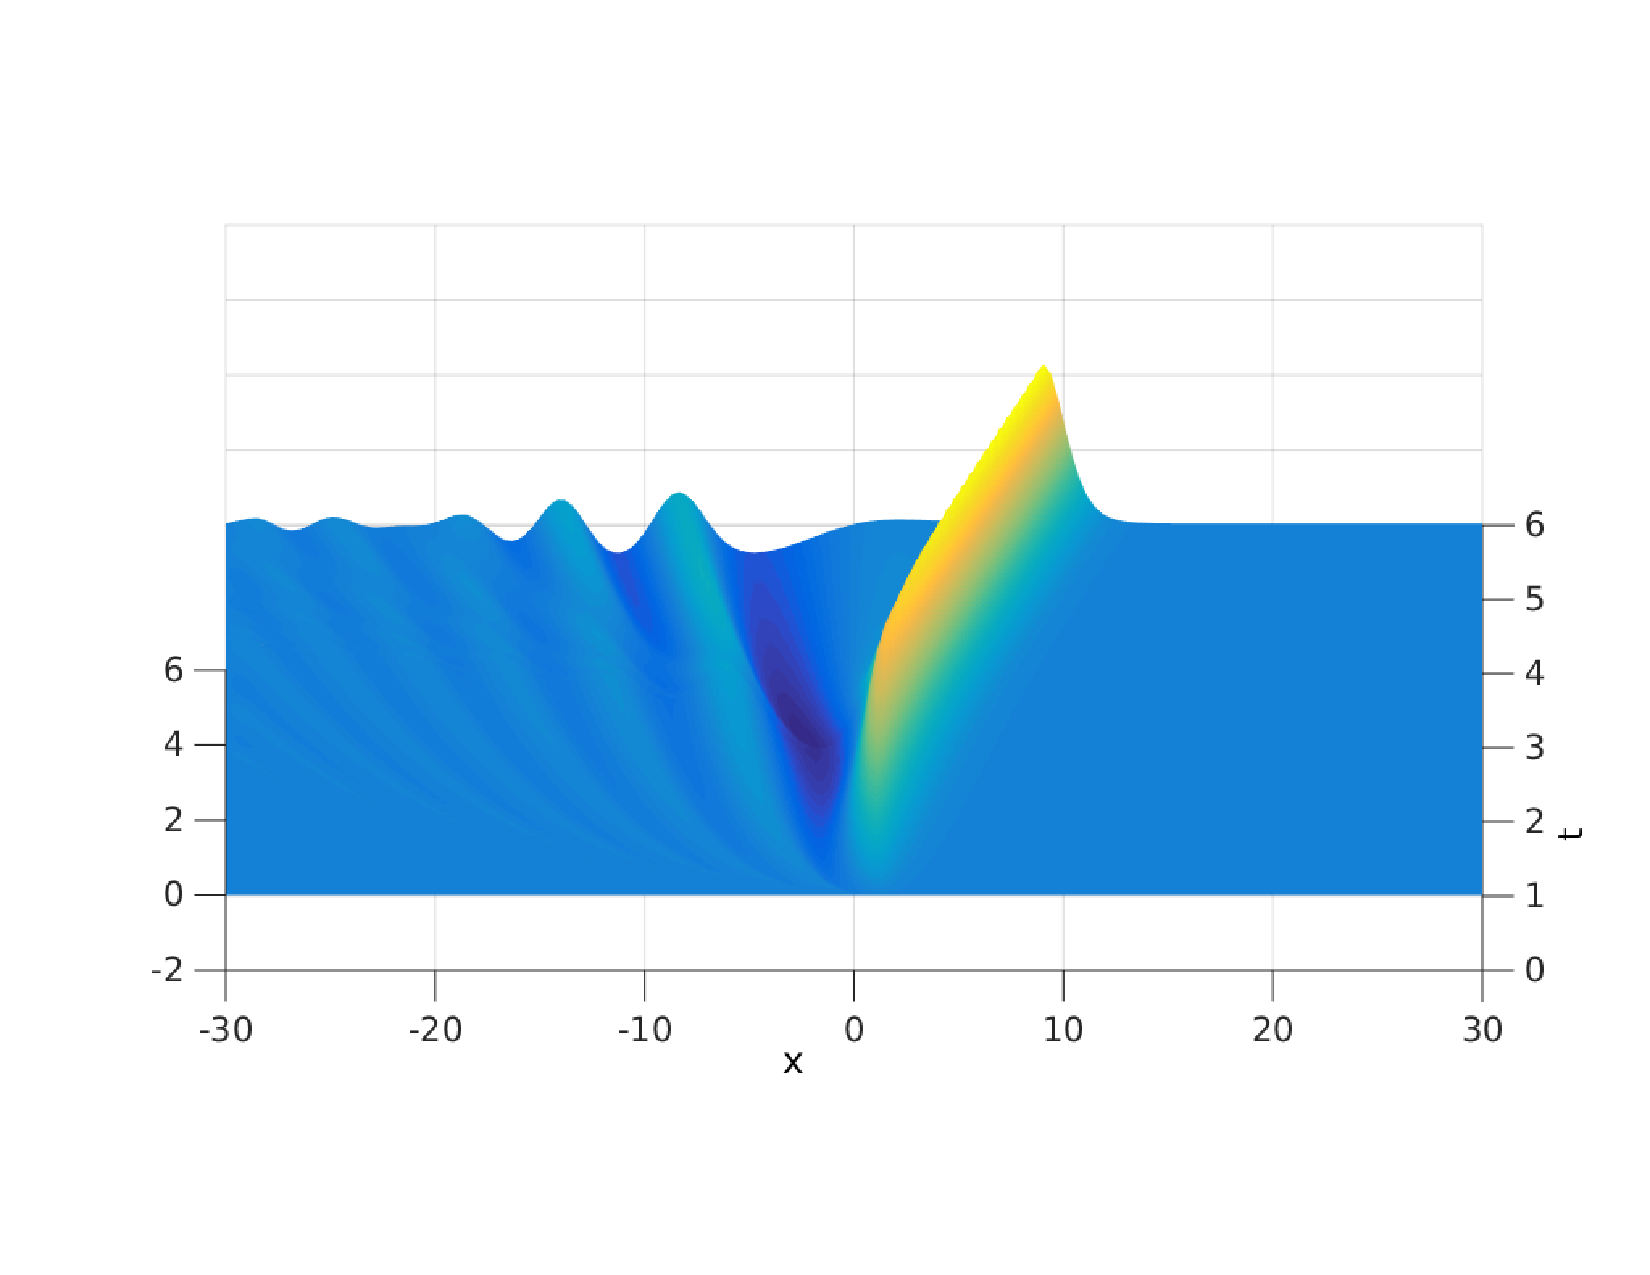
\includegraphics[width = 0.45\textwidth]{images/ex1yd3D.pdf}
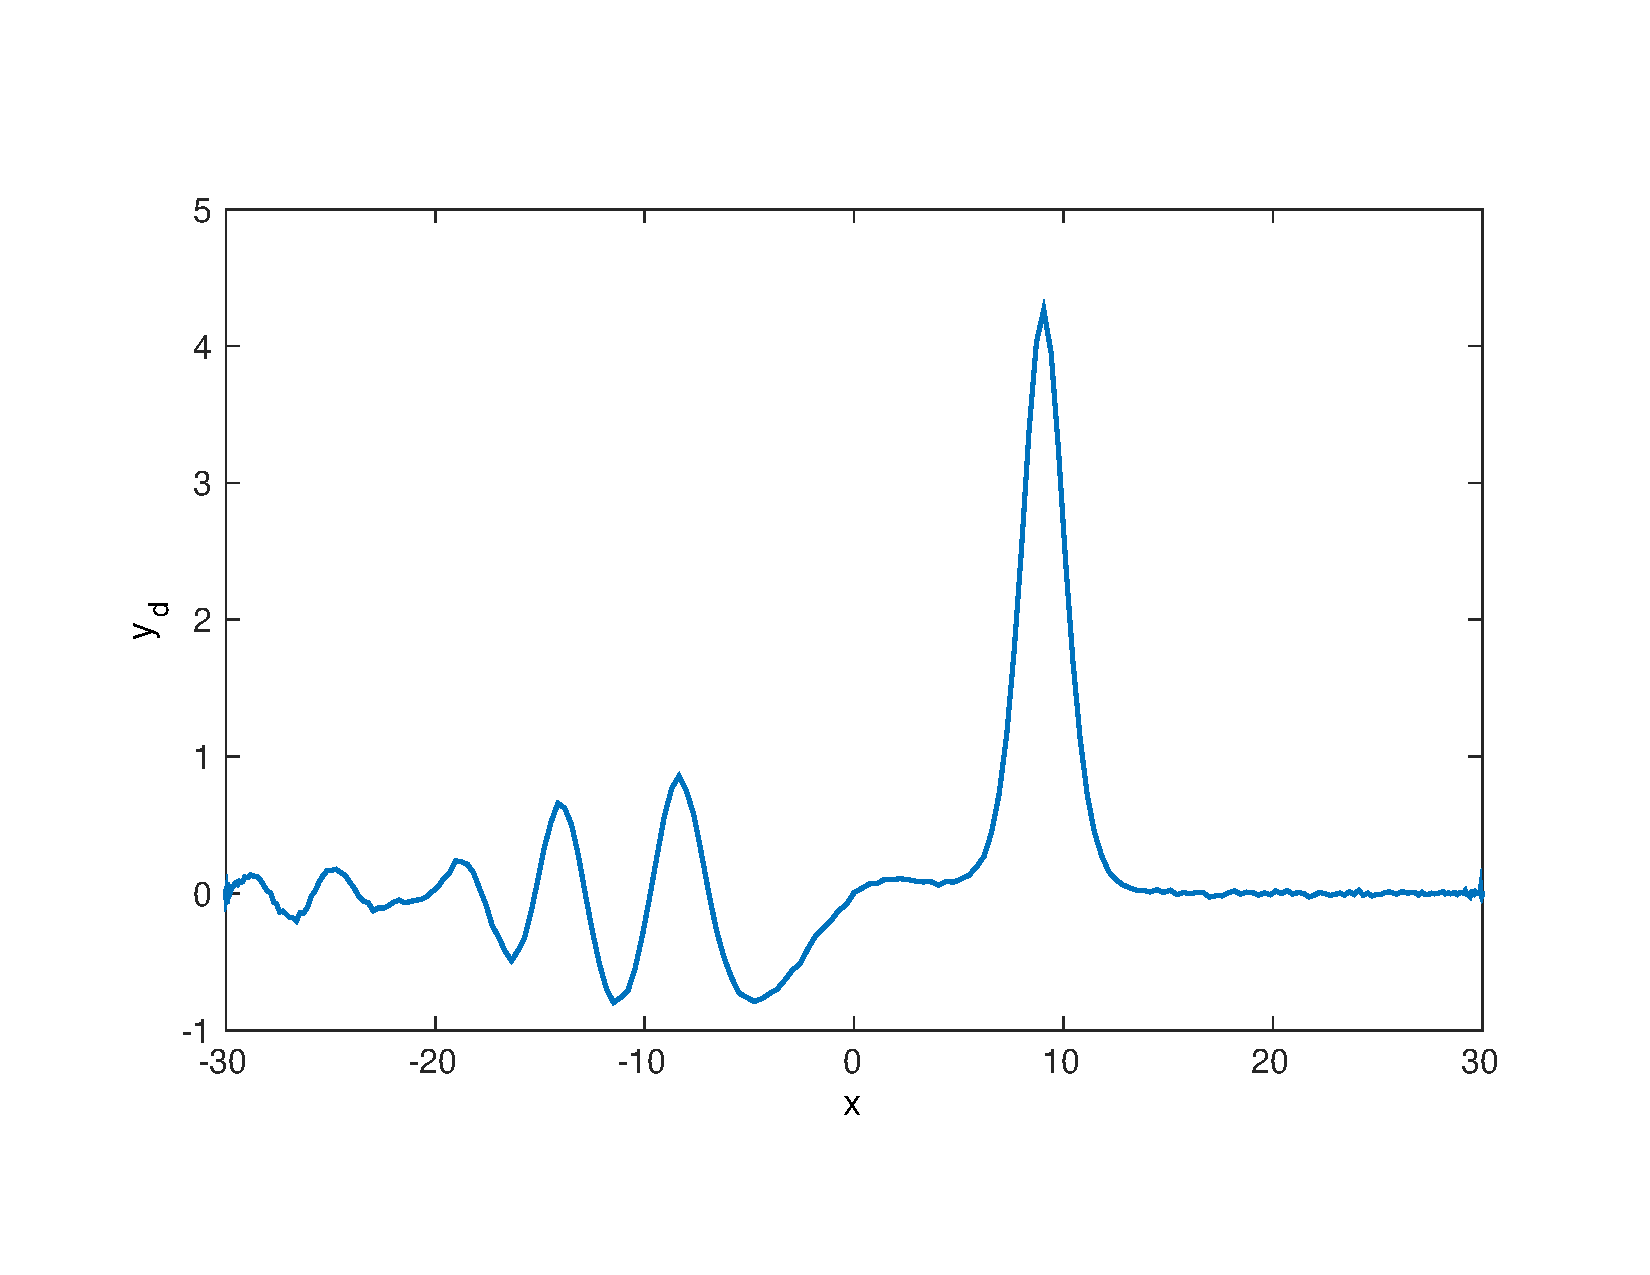
\includegraphics[width = 0.45\textwidth]{images/ex1yd.pdf}
\caption{Left: wave generated by the forcing term $u$, for $f = -0.5$ (i.e. subcritical flow). Right: $y$-profile at final time with Gaussian white noise.}
\label{waveobservation}
\end{figure}

At the end of the continuation strategy, the support of the control is, according to Proposition~\ref{propsubgcondition}, included in the domains where $\|q\|_{L^2(I)} = \frac{\alpha}{\gamma}$. One can see on Fig.~\ref{support} that the final control is a point source, located at the exact right position. The time profile of the control is depicted on Fig.~\ref{recoveredcontrol} and follows the original one quite well. One points out that the oscillations are due to the noise. It enters indeed directly as an initial condition in the adjoint equation and is not filtered in any manner on the support of the control, where \eqref{controlintime} holds for the time profile of $u$.
\begin{figure}[!h]
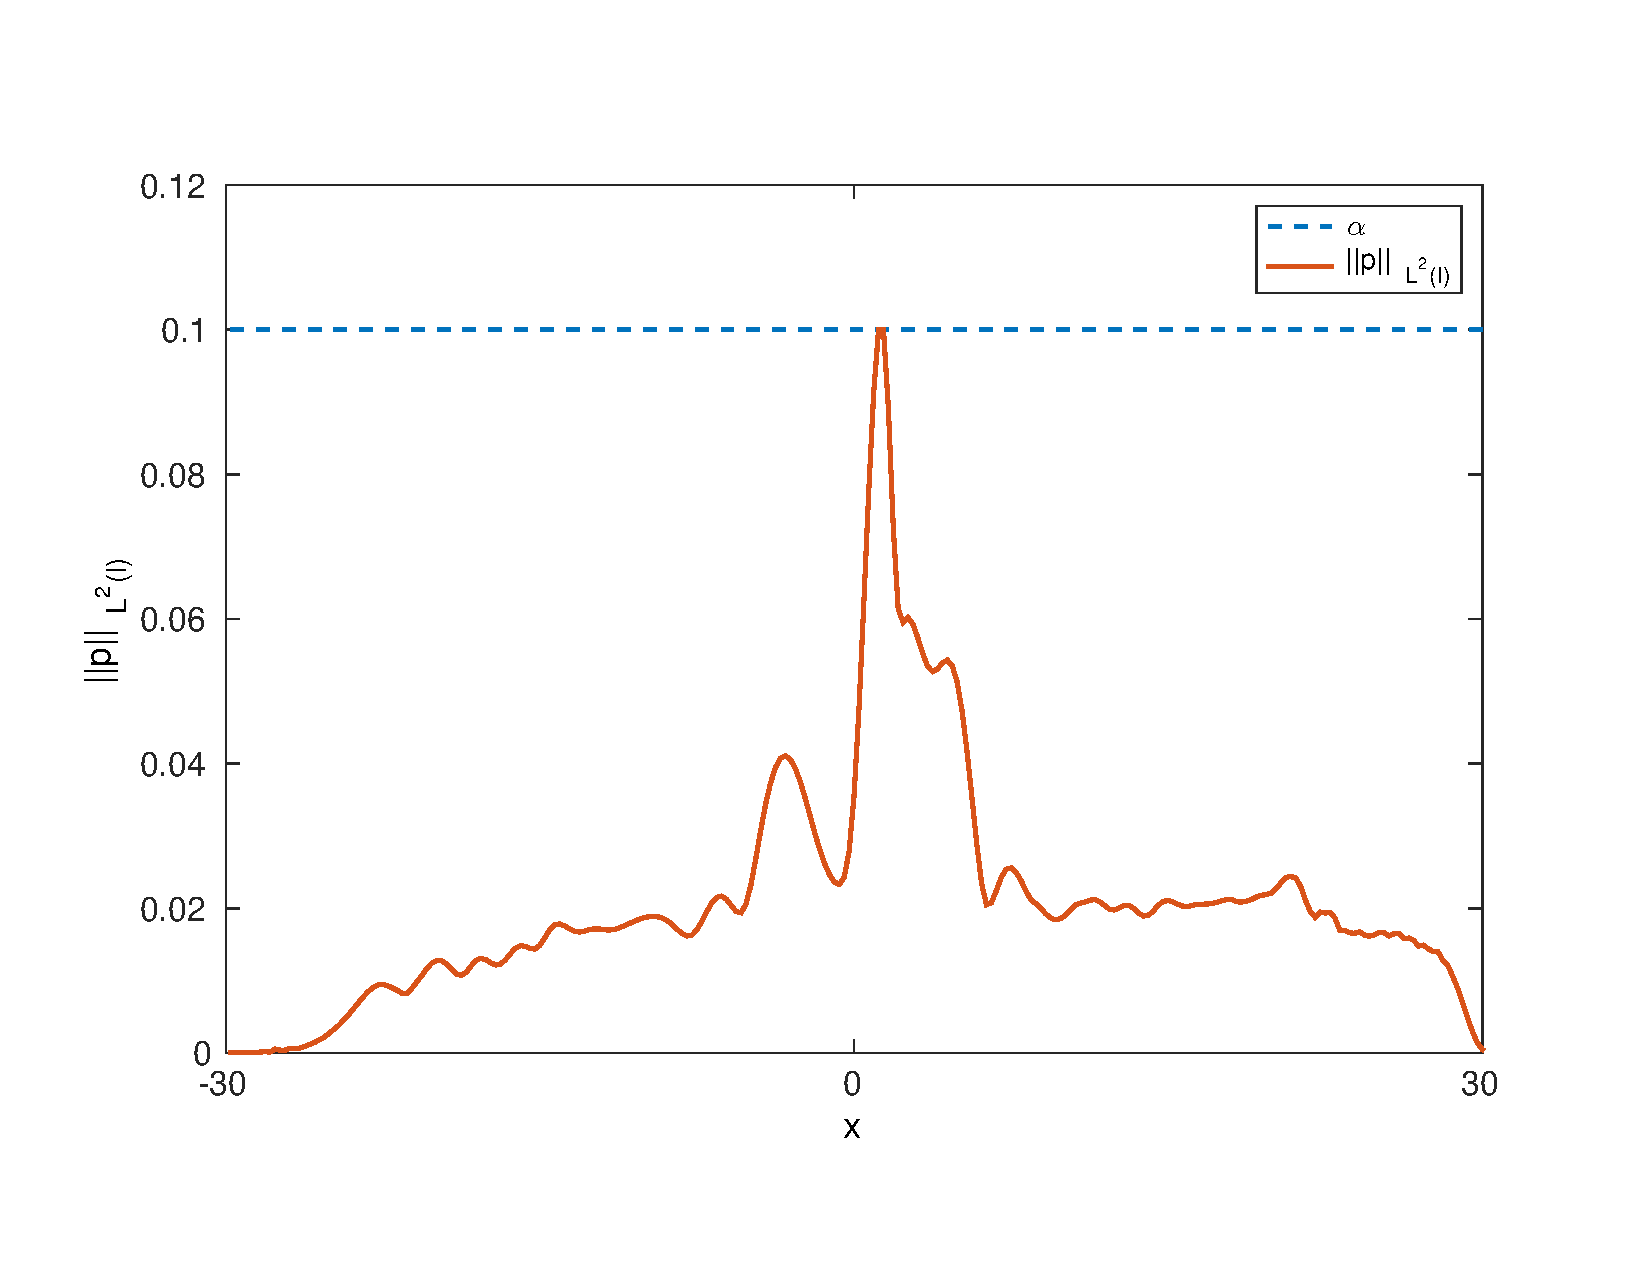
\includegraphics[width = 0.75\textwidth]{images/normp.pdf}
\caption{Spatial support of the control, determined by $\norm{q}_{L^2(0,T)}\geq \frac{\alpha}{\gamma}$. Here $\alpha = 0.1$ and $\gamma = 10^{-6}$}
\label{support}
\end{figure}
\begin{figure}[!h]
 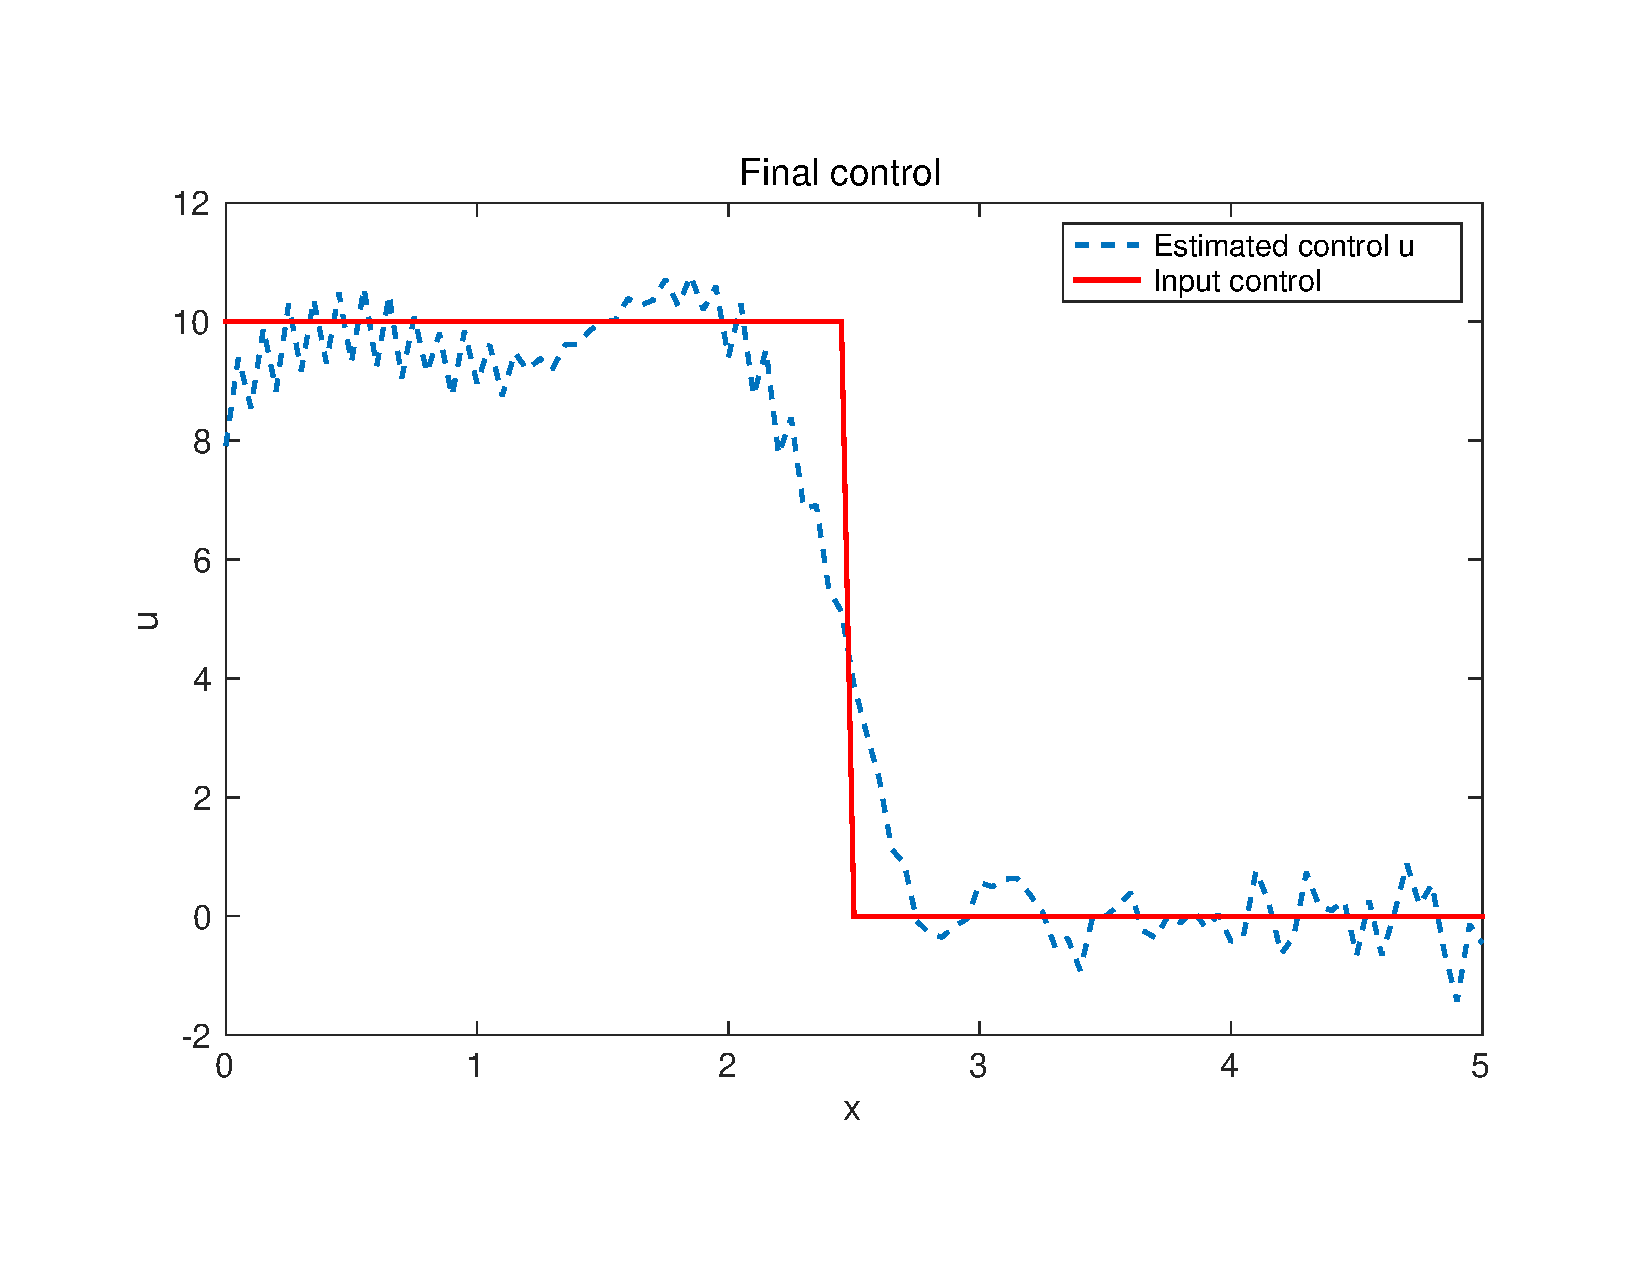
\includegraphics[width = 0.75\textwidth]{images/ex1recoveredcontrol2.pdf}
 \caption{Recovered control for $\gamma = 10^{-6}$}
 \label{recoveredcontrol}
\end{figure}
The results  of the optimization process are shown on Fig.\ref{recoveredstate}, for $\alpha = 0.1$.
\begin{figure}[!h]
 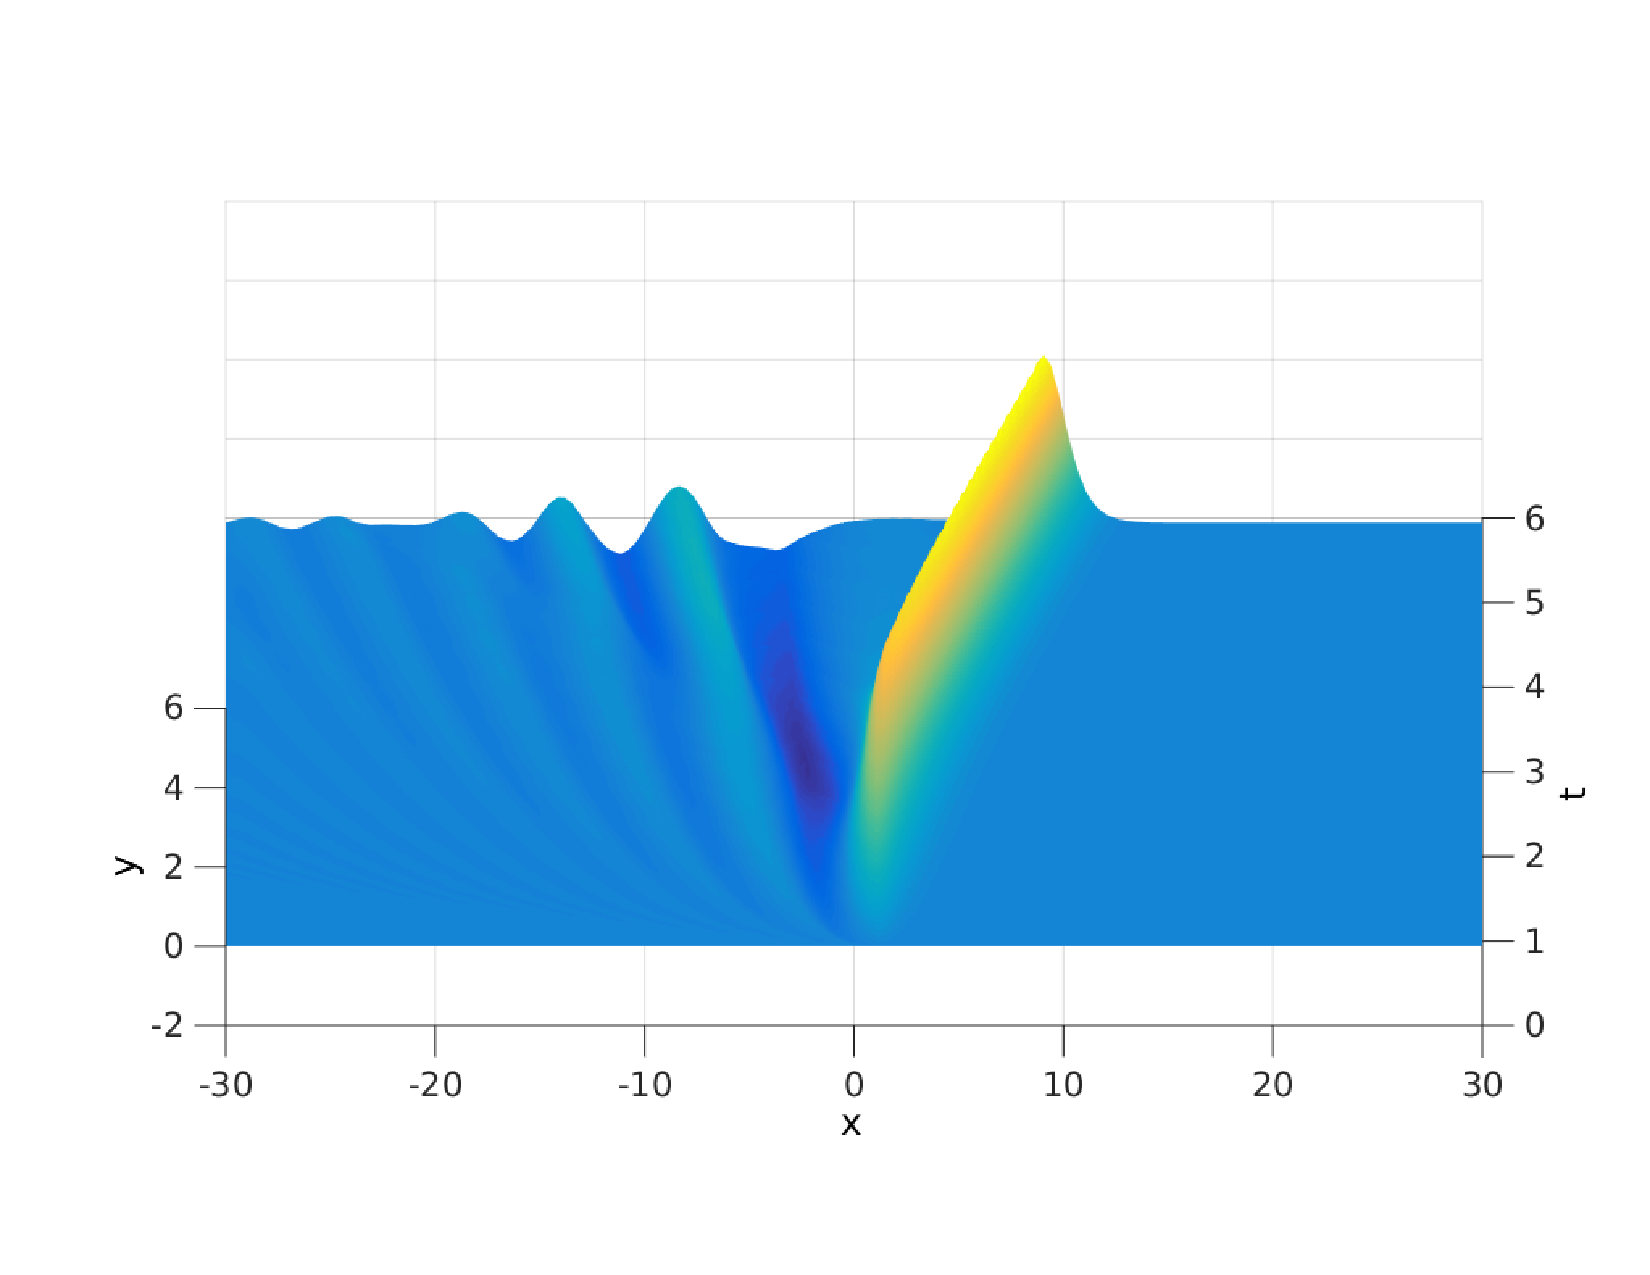
\includegraphics[width = 0.45\textwidth]{images/ex1recoveredstate3d.pdf}
  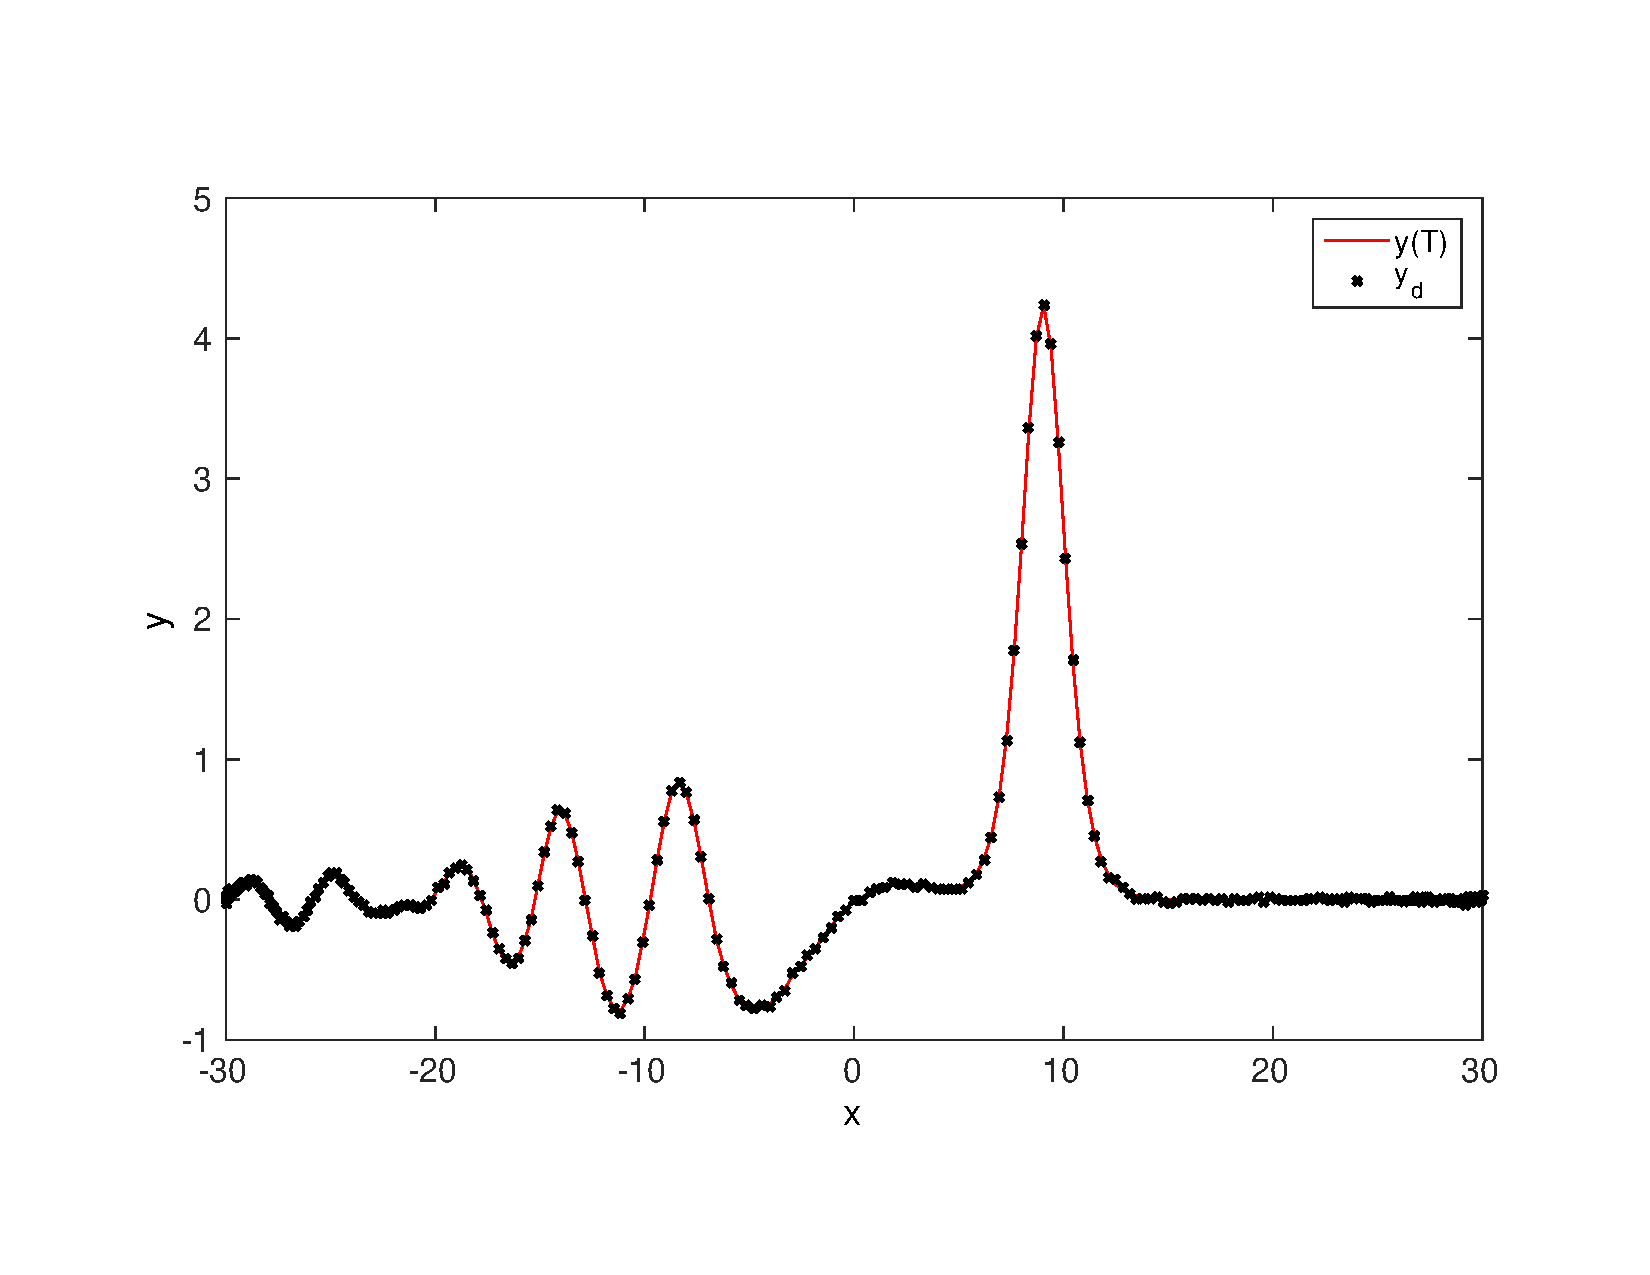
\includegraphics[width = 0.45\textwidth]{images/ex1recoveredstate.pdf}
 \caption{Recovered state $y$ and final observation $y(T)$ for $\gamma = 10^{-6}$}
 \label{recoveredstate}
\end{figure}

\paragraph{\underline{Control example}.}
The second example is a control example. We divide the domain $\Omega = [-L,L]$ into two subdomains. The domain $\Omega_c = [-L,0]$ is the control domain, while $\Omega_{obs} = [0,L]$ is the observation domain. See Fig.~\ref{controlsetup} for the description of the setup. The flow enters the domain from the right and we want to create the wave profile shown on Fig.\ref{objectivewave} on $\Omega_{obs}$, acting only on $\Omega_c$.
\begin{figure}[!h]
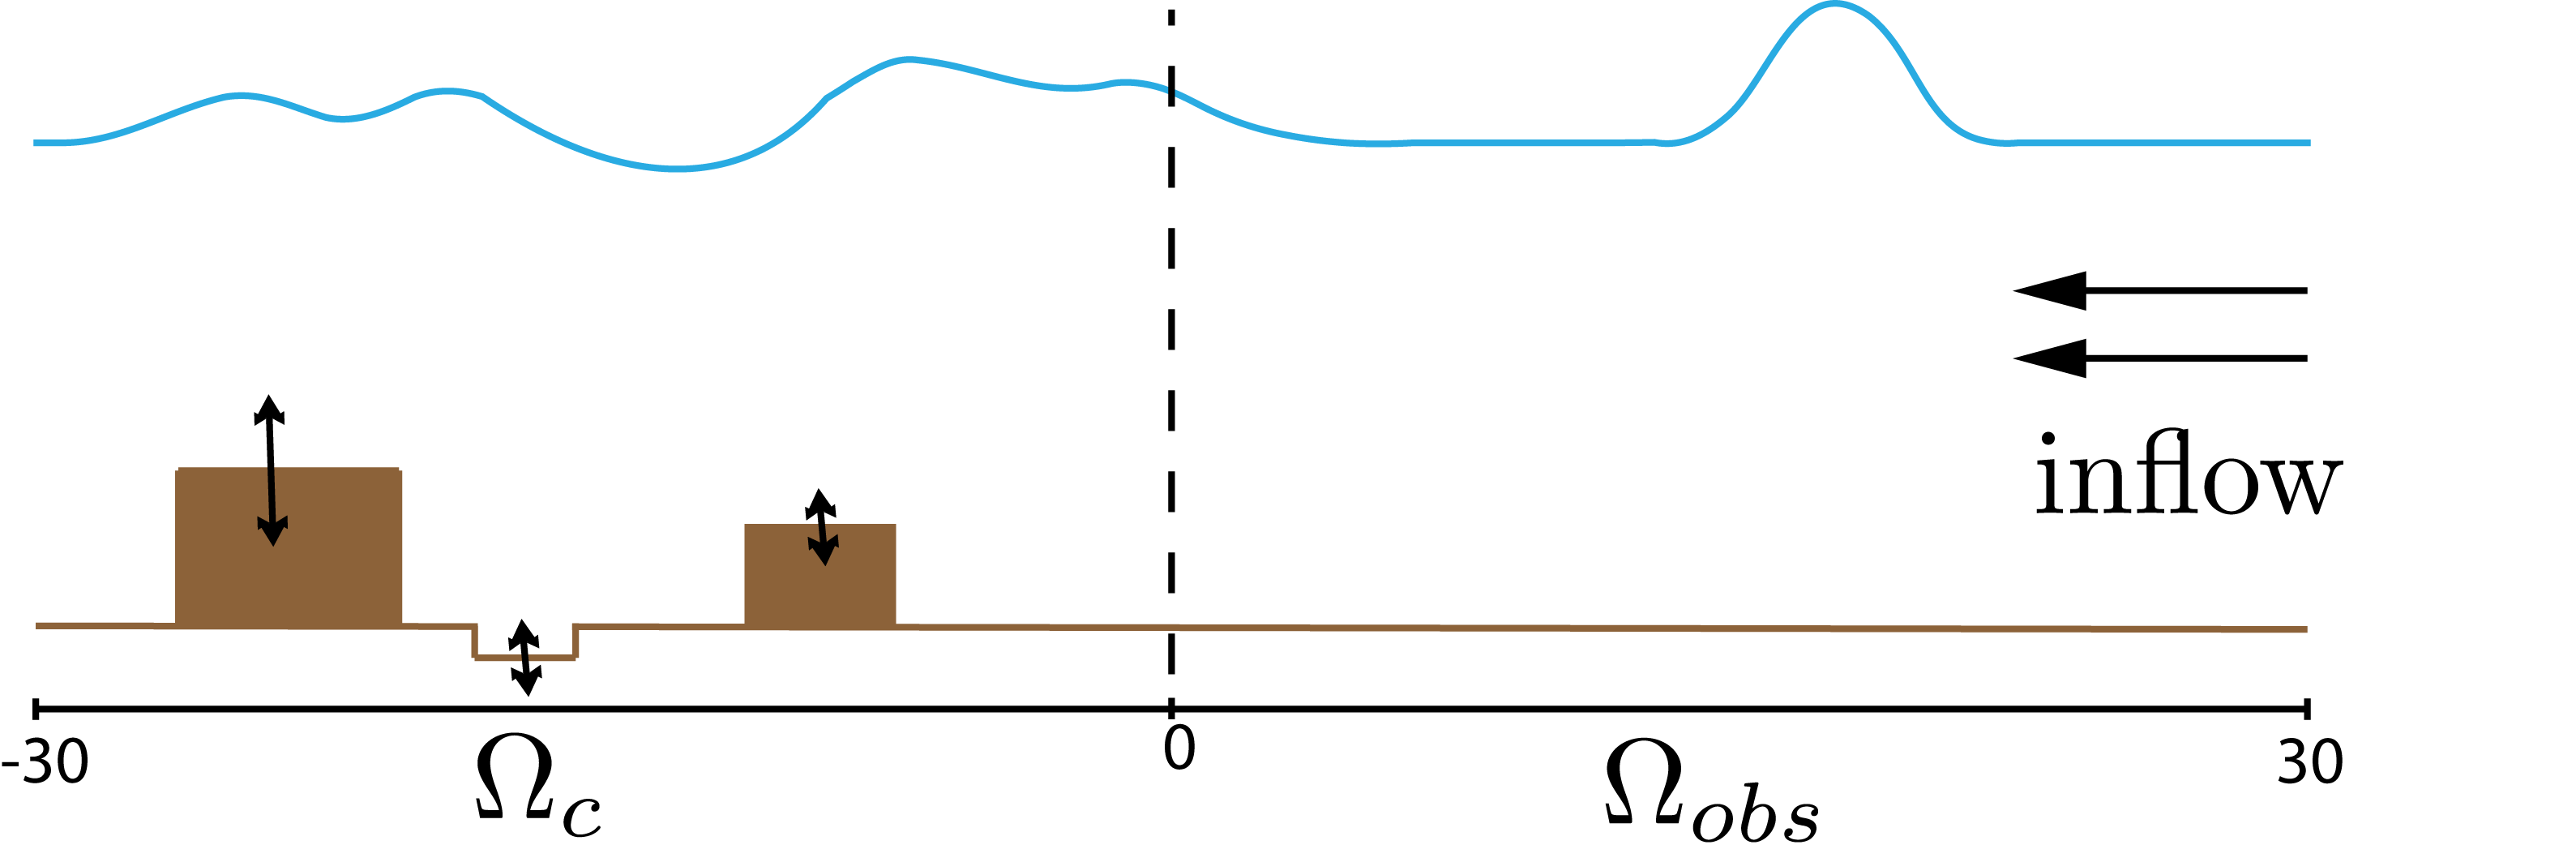
\includegraphics[width = 0.75\textwidth]{images/control_setup.png}
\caption{Setup of the control problem.}
\label{controlsetup}
\end{figure}
\begin{figure}[!h]
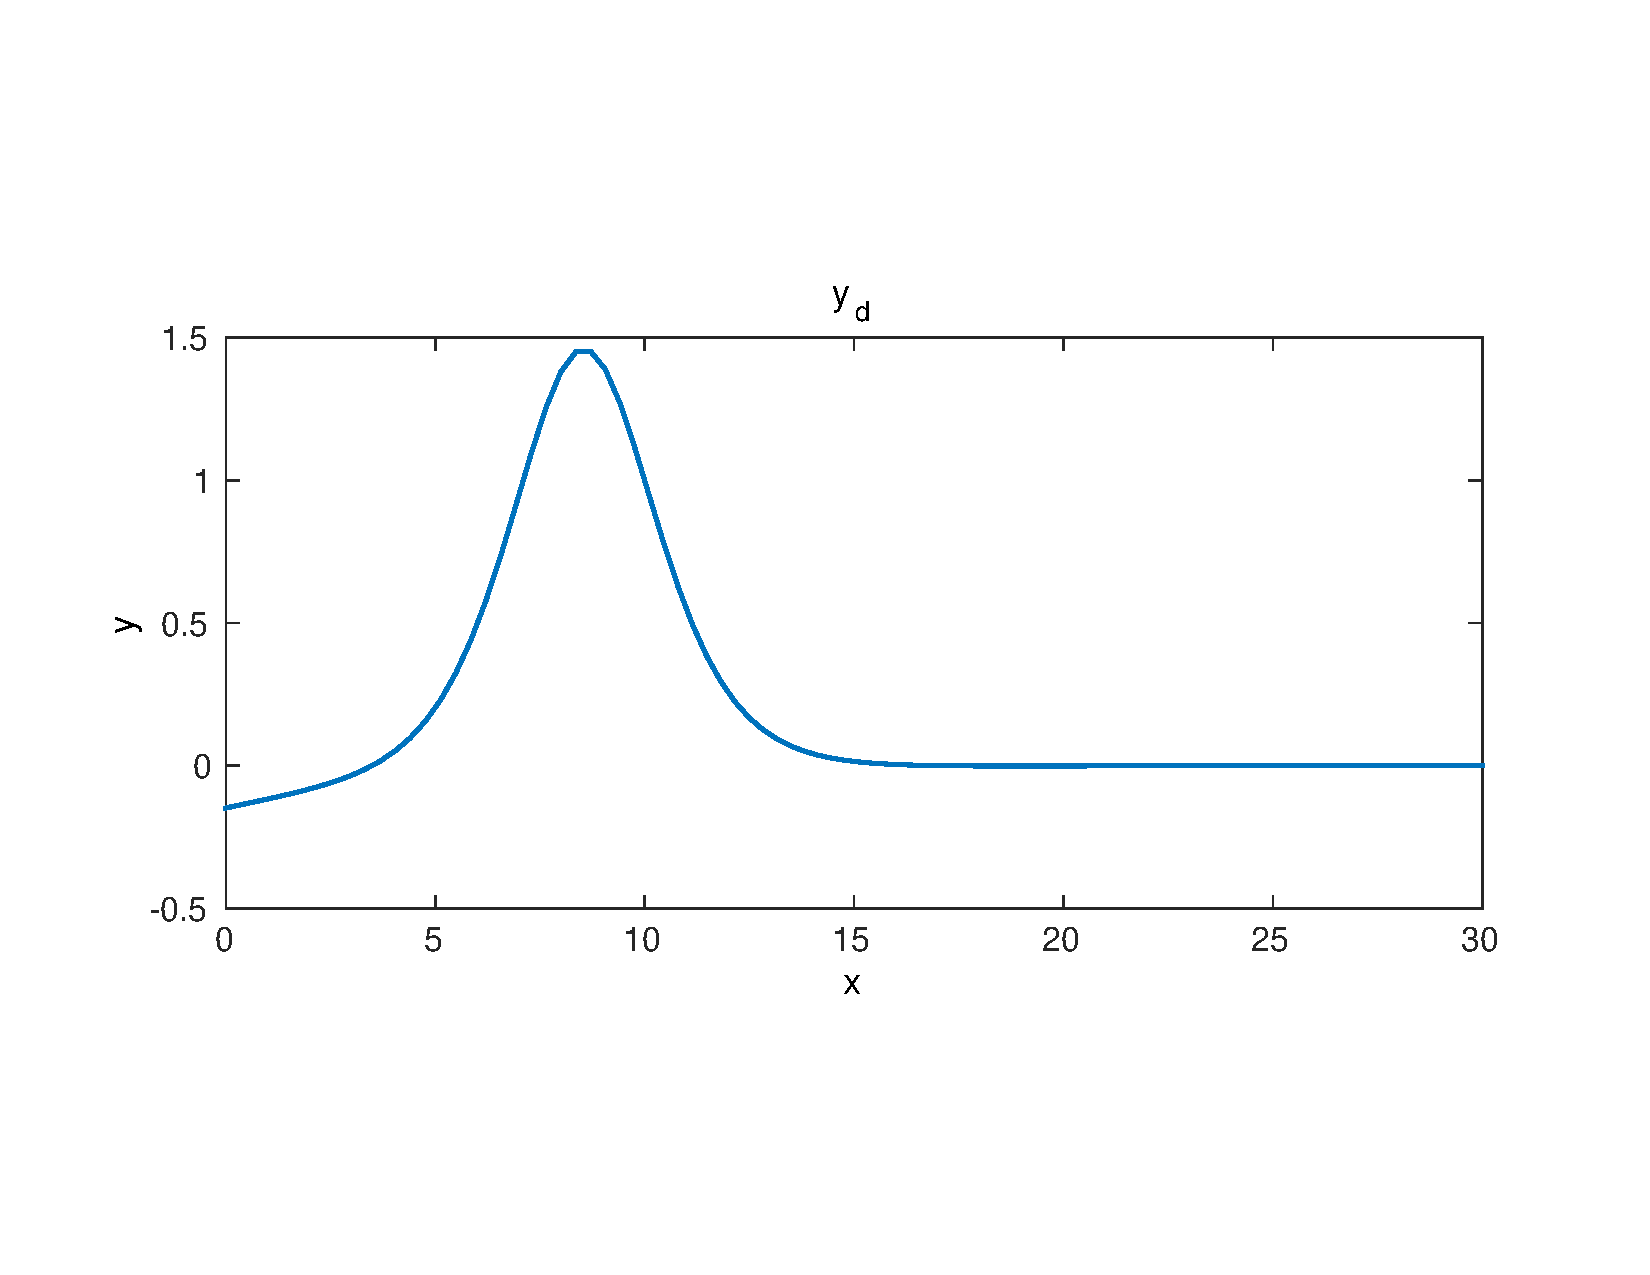
\includegraphics[width = 0.75\textwidth]{images/ex2yd.pdf}
\caption{Objective wave at final time T.}
\label{objectivewave}
\end{figure}
The support of the control is depicted on Fig.~\ref{supportIP}. At the end of the continuation strategy, it boils down to two point sources. One can see clearly on Fig.~\ref{recoveredcontrol} that it has smooth variations in time, as induced by the $L^2$ norm. The optimized state is shown on Fig.~\ref{ex2fullgammadm5} for $\gamma = 10^{-5}$. An upstream going soliton is created that matches accurately at final time the objective wave. Naturally, spurious waves are created on the control domain that do not have to be avoided since they are not observed.
\begin{figure}[!h]
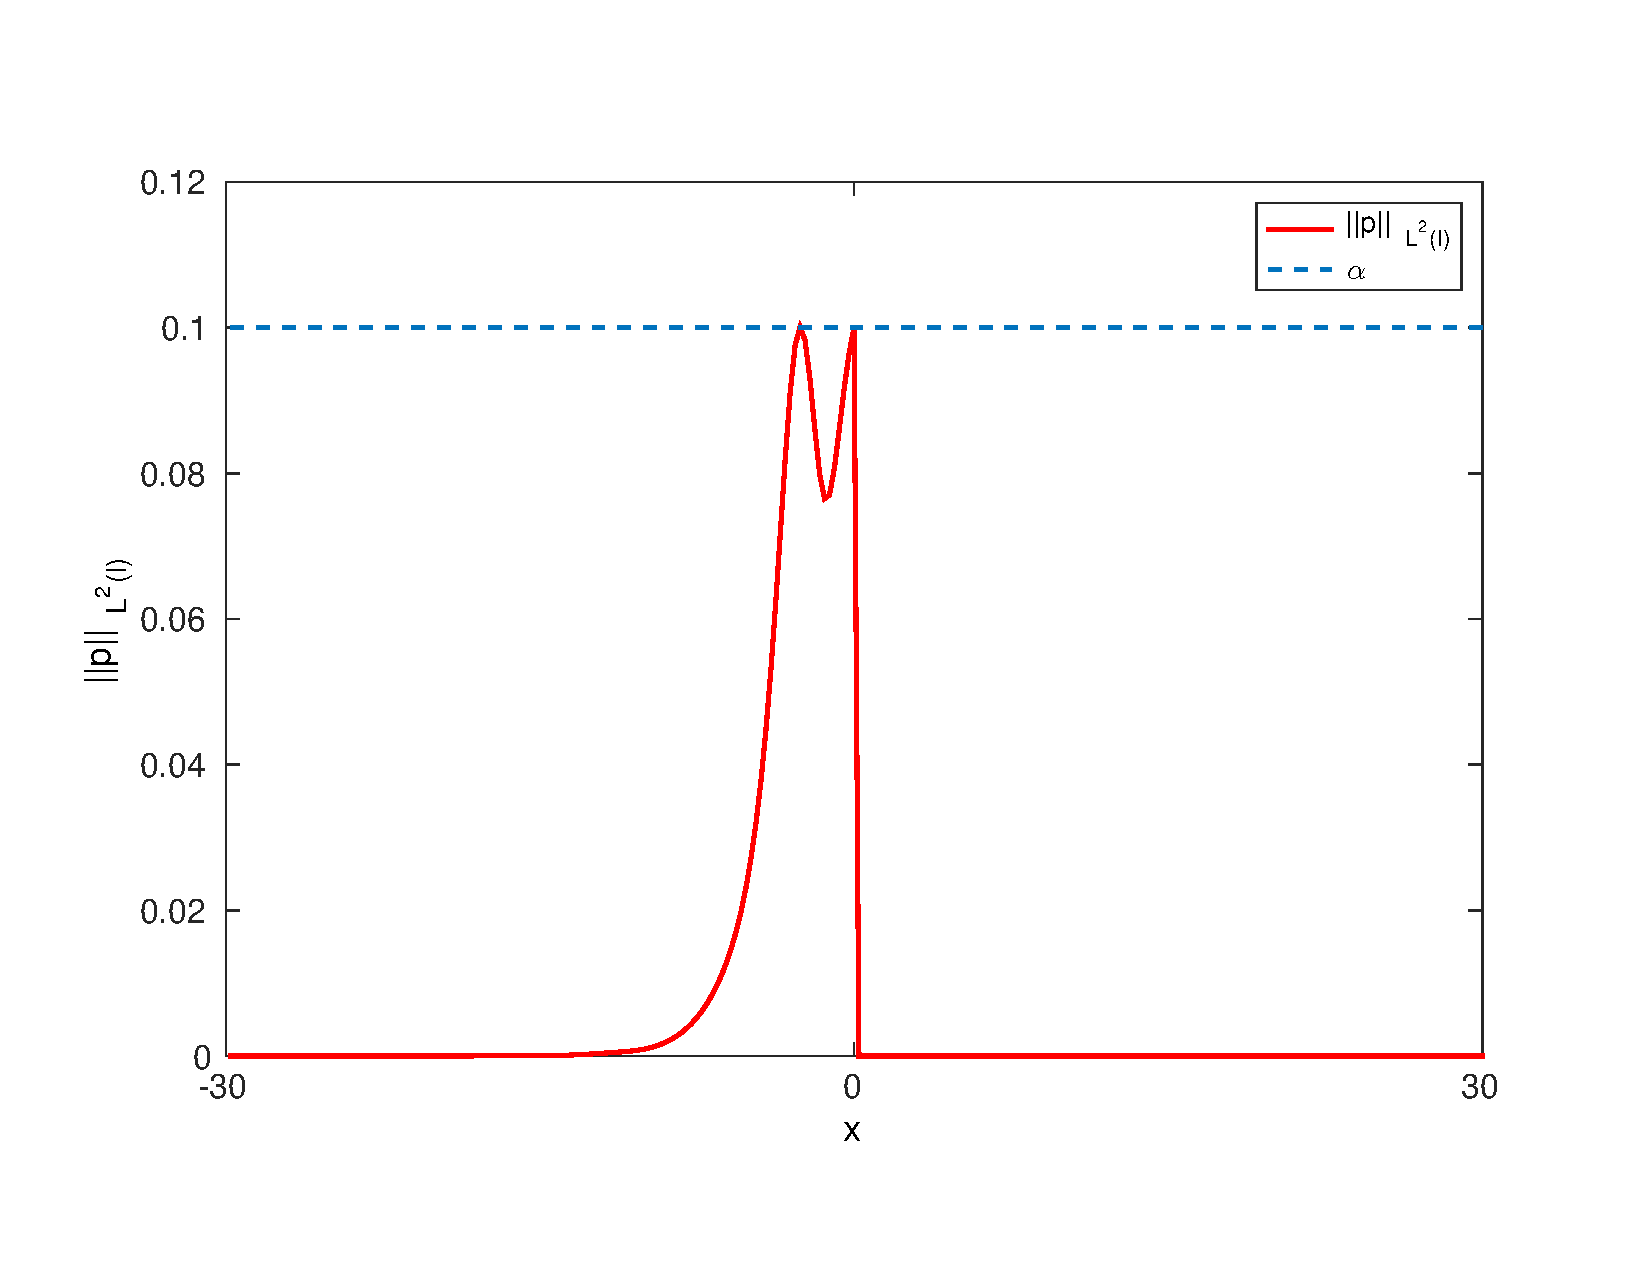
\includegraphics[width = 0.75\textwidth]{images/norm2p.pdf}
\caption{Spatial support of the control, determined by $\norm{q}_{L^2(0,T)}\geq \frac{\alpha}{\gamma}$, for $\gamma = 10^{-5}$.}
\label{supportIP}
\end{figure}

\begin{figure}[!h]
 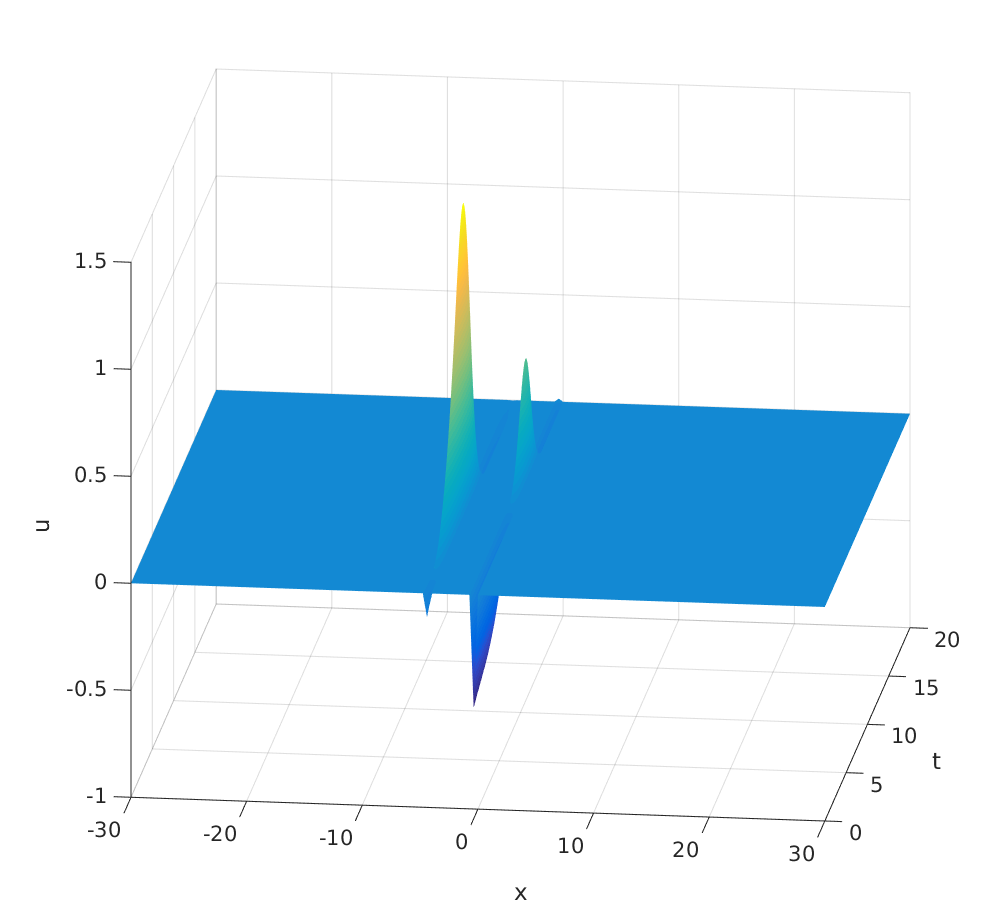
\includegraphics[width = 0.45\textwidth]{images/ex2optcontrol3d.png}
 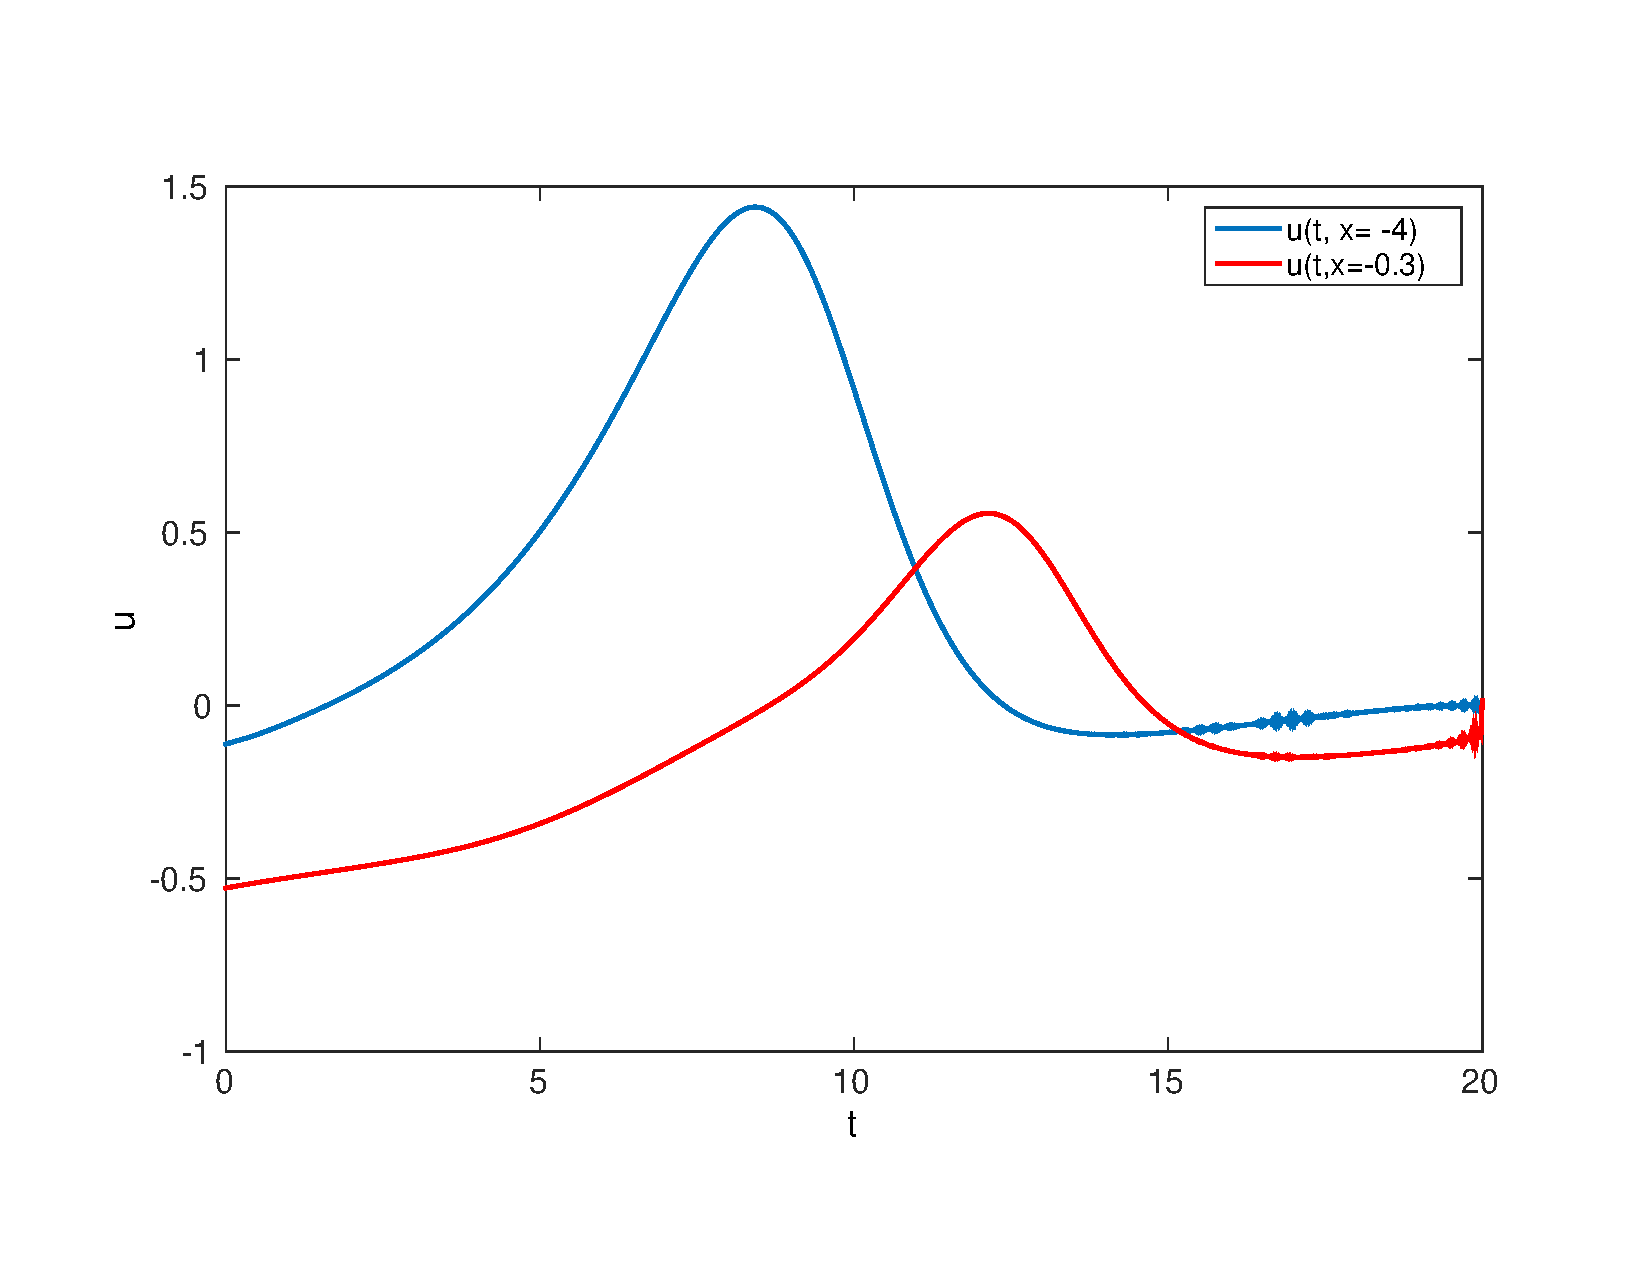
\includegraphics[width = 0.45\textwidth]{images/ex2utime.pdf}
 \caption{Optimal control $u$, $\gamma = 10^{-5}$}
 \label{recoveredcontrol}
\end{figure}


\begin{figure}[!h]
 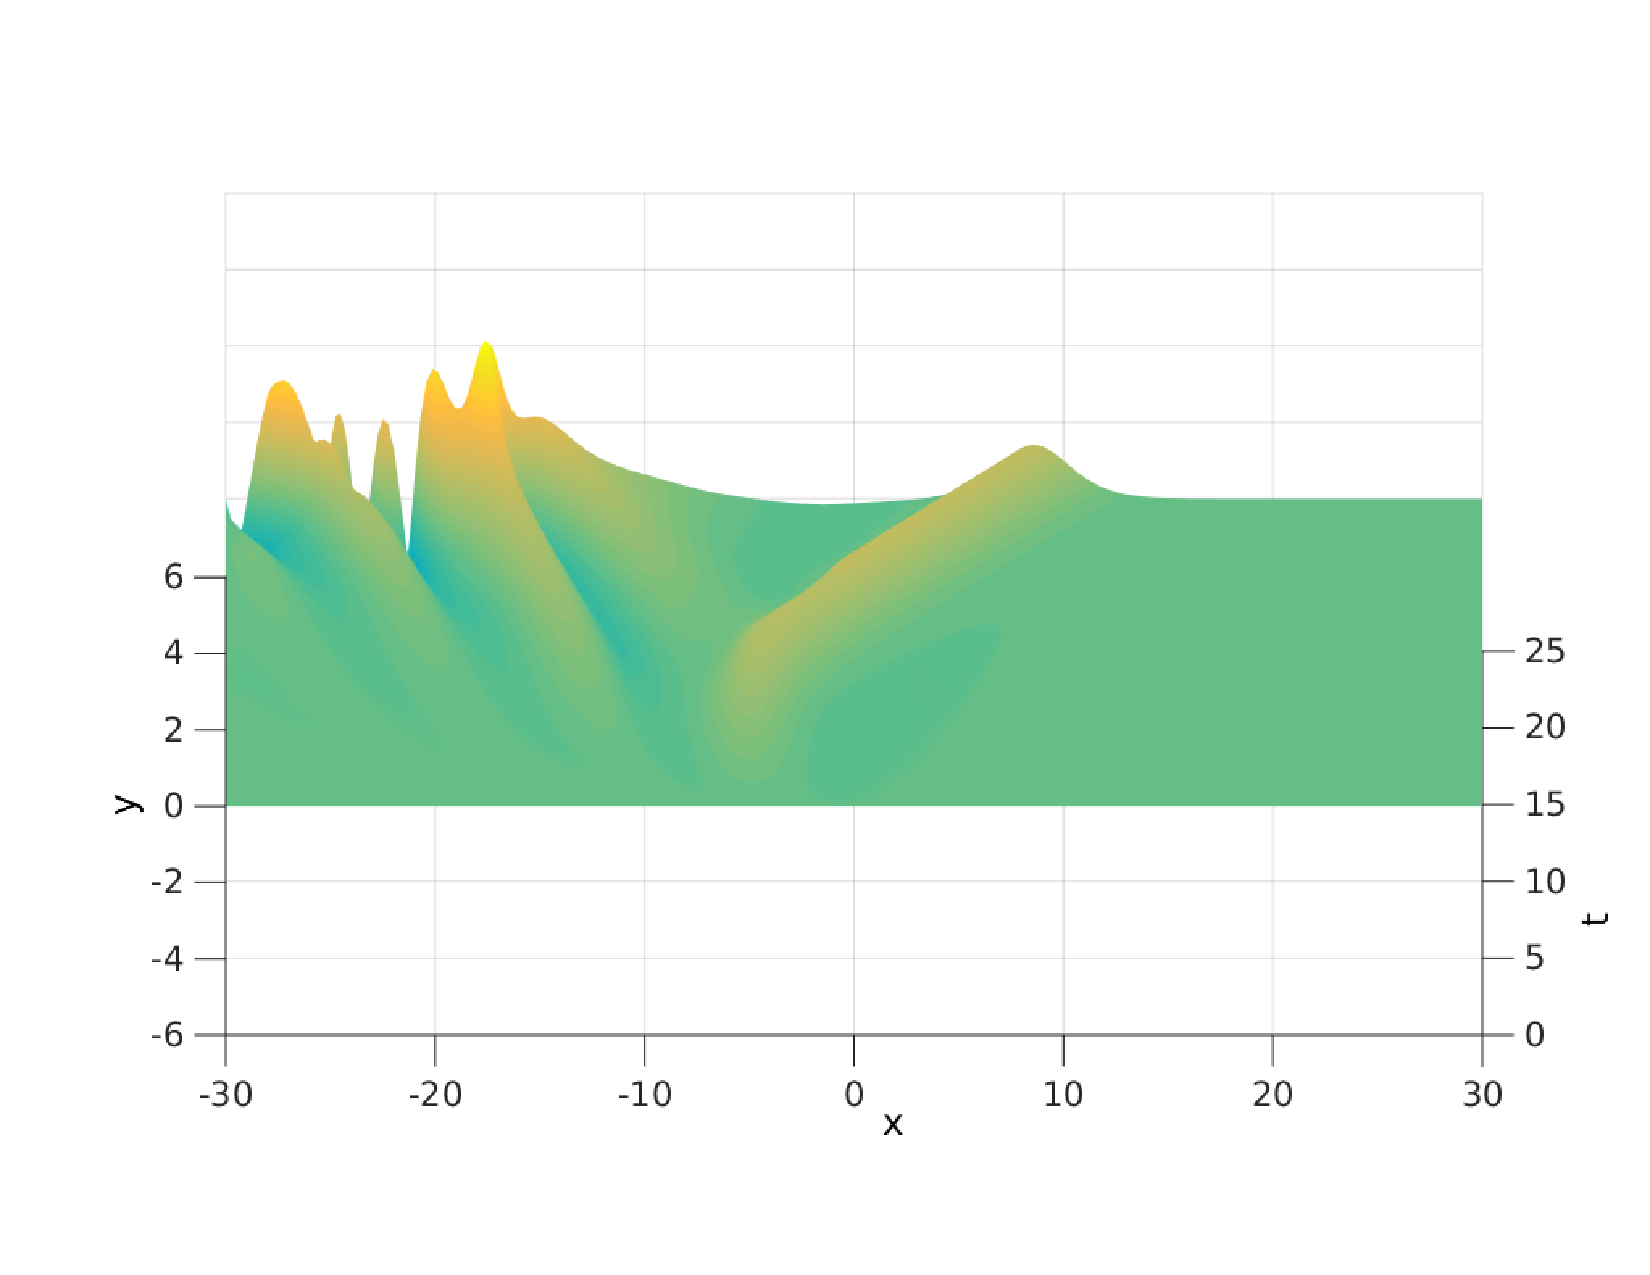
\includegraphics[width = 0.45\textwidth]{images/ex2state3d.pdf}
 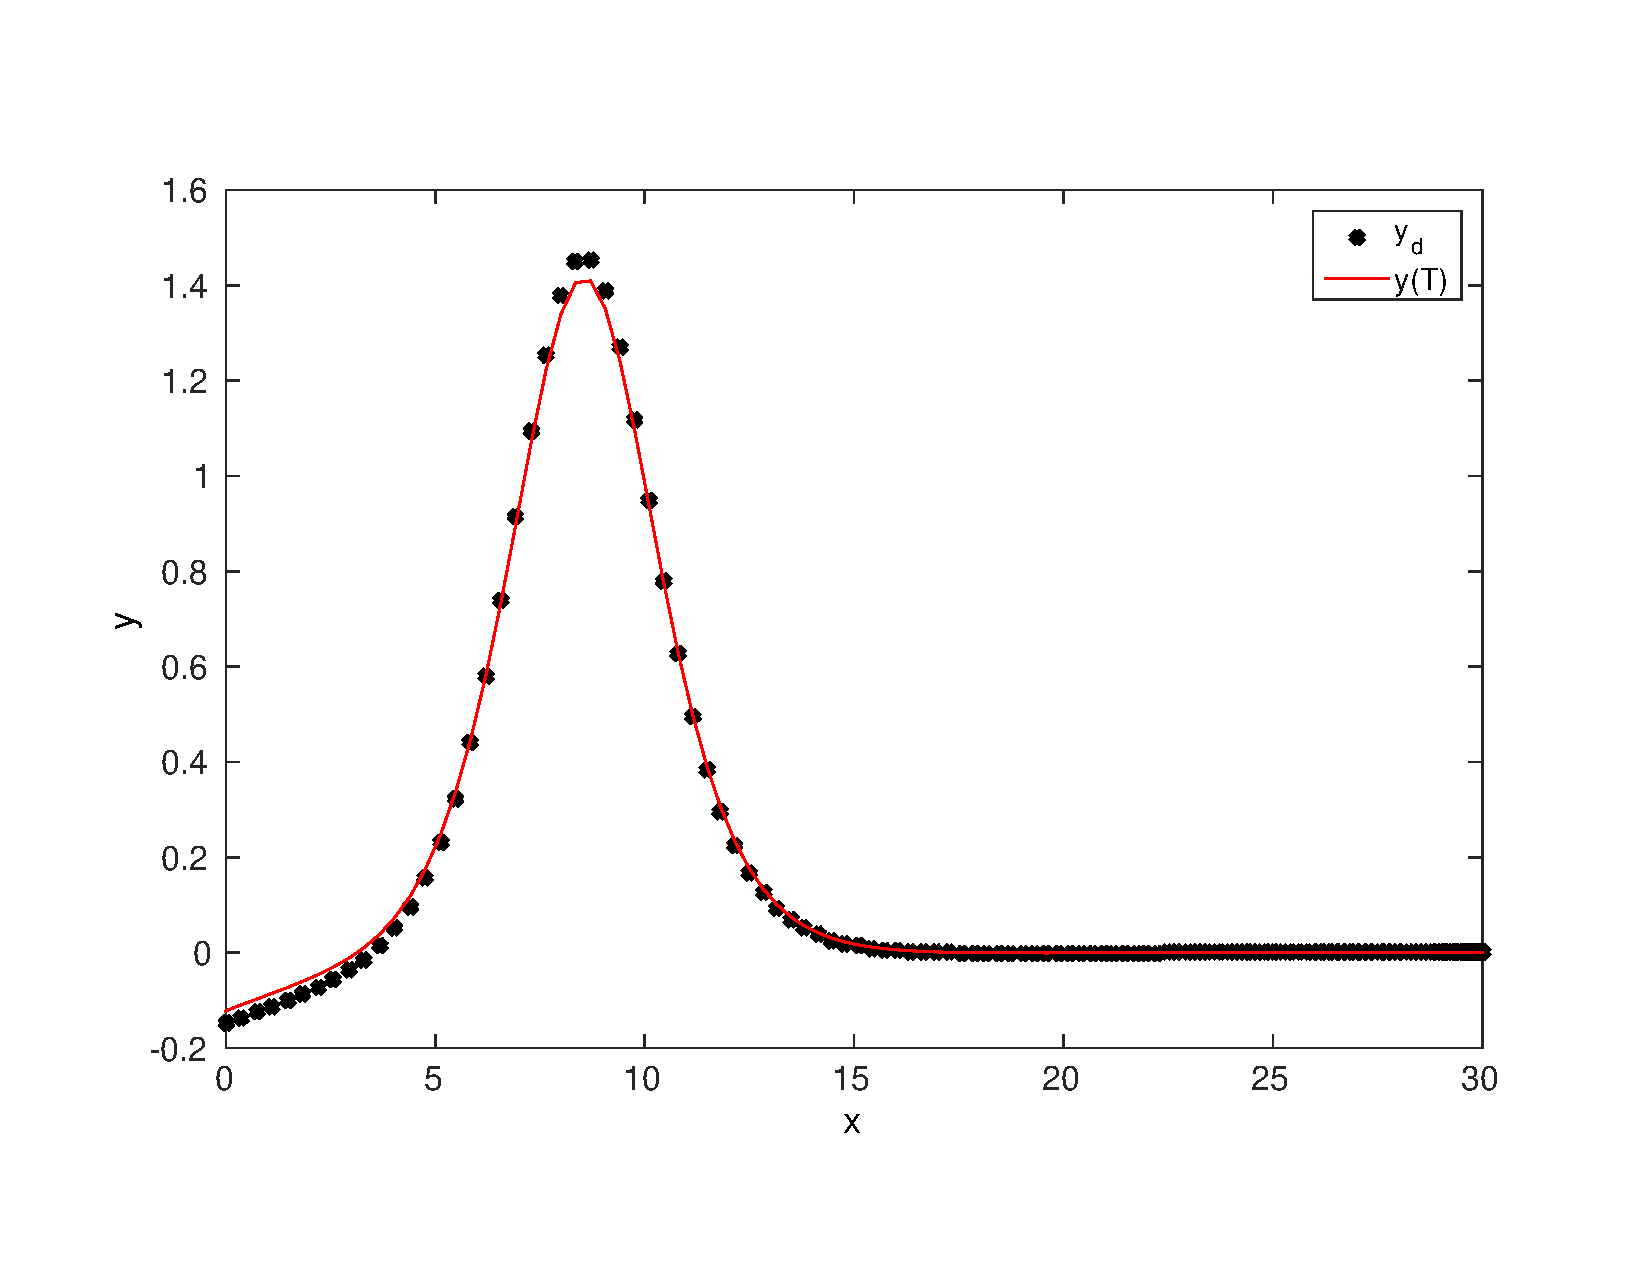
\includegraphics[width = 0.45\textwidth]{images/controlledstate.pdf}
 \caption{Left: evolution of the optimized state y for $\gamma = 10^{-5}$. Right: final optimized state y(T), compared with the objective shape for $\gamma = 10^{-5}$.}
 \label{ex2fullgammadm5}
\end{figure}


\clearpage

%%% Local Variables:
%%% mode: latex
%%% TeX-master: "kdv.tex"
%%% End: 